%% Supplementary Material for
%%   "Measuring Counseling Interaction Patterns Across Human--Human and Human--LLM Dialogues"
%% Standalone companion document -- tables and figures are numbered S1, S2, ...
%% Build: pdflatex -interaction=nonstopmode oncoco_supplementary.tex   (twice; no bibliography)

\documentclass[fleqn,10pt]{JLA_article}

\usepackage[american]{babel}
\usepackage{csquotes}

\newcommand{\fitwidth}[1]{\resizebox{\ifdim\width>\linewidth \linewidth\else \width\fi}{!}{#1}}
% role-specific proximity gaps: Delta = JSD(HH real, H-LLM) - JSD(HH real, HH roleplay)
\newcommand{\dCL}{\Delta_{\mathrm{CL}}}
\newcommand{\dCO}{\Delta_{\mathrm{CO}}}
\setlength{\emergencystretch}{3em}

% S-prefixed numbering so references from the main paper are unambiguous
\renewcommand{\thesection}{S\arabic{section}}
\renewcommand{\thetable}{S\arabic{table}}
\renewcommand{\thefigure}{S\arabic{figure}}

\PaperTitle{Supplementary Material: Measuring Counseling Interaction Patterns Across Human--Human and Human--LLM Dialogues}
\Authors{}
\affiliation{}
\Keywords{}
\Submitted{} \Accepted{} \Published{}
\Volume{} \Number{} \Pages{} \Doi{}
\WithoutNotestrue
\Abstract{This document accompanies the main article. It reports the full persona list, complete client- and counselor-side OnCoCo label distributions, hidden-Markov state summaries and state-count sensitivity, transition heatmaps, sentence-embedding projections, per-conversation within-condition variability, the RQ2 multiplicity control, the noise-band placement under each unit of analysis, the classifier-confidence diagnostics, the pre-declared category exclusion sets with their leave-one-out sweep, the unit-of-analysis table, and the prompt-replay experiment of RQ3. Tables and figures are numbered S1, S2, \ldots and are referenced by those numbers in the main text.}

\begin{document}

\flushbottom
\maketitle
\thispagestyle{fancy}

\section{Prompts and Case Descriptions}
\label{Ssec:prompts}
The prompt templates that drove the simulated client are released in the companion repository (directory \texttt{prompts/}), one file per persona and template variant, with the conversation history that the platform inserts at generation time replaced by a placeholder. The repository also contains the HH roleplay and H--LLM conversations with personal data masked, the OnCoCo labels aligned to the masked text, the persona definitions, and the segmentation adapter. Prompts of the earliest deployment (Mixtral 8x7B) were not logged by the platform at that time. HH real conversations are not released because they stem from real help-seekers.

The platform assembles each prompt from a persona profile and one of two template families. Plain-text templates open with a role instruction (``\# Rollenanweisung'' for the first turn, ``Du bist \ldots'' for later turns).
Chat-template prompts wrap the same persona in the Llama~3 chat format with a structured ``\#\# Antwortformat'' block. Every logged template carries a brevity instruction at template level (``Maximal 1-2 kurze S\"atze'', ``1-4 S\"atze maximal'', ``kurz und pr\"azise''), so the only brevity cue that varies between conversations is the persona profile's ``Sprachliche Merkmale'' field (e.g.\ ``Kurze pr\"agnante R\"uckmeldungen''). Ten of the 26 personas in the analysed H--LLM conversations carry such a cue. Table~\ref{Stab:prompt-variants} reports the client-side distance to HH real per prompt configuration, Table~\ref{Stab:verbosity} the message-length and punctuation statistics behind the verbosity signature, and Table~\ref{Stab:sizematched} the size-matched subsample check.

\section{Persona List}
\label{Sapp:personas}
\begin{table}[t]
\caption{Personas used in chat roleplays (short descriptions truncated to the first sentence).}
\label{Stab:personas}
\centering
\small
\setlength{\tabcolsep}{3pt}
\begin{tabular}{r p{0.24\linewidth} r p{0.52\linewidth}}
\toprule
\# & Persona name(s) & Conv. & Case brief (first sentence) \\
\midrule
1 & Luisa & 89 & Luisa ist genervt von den Streitereien ihrer Eltern. \\
2 & Michael Schlosser & 70 & Herr Schlosser m\"ochte gerne wieder eine Arbeit finden. \\
3 & Elke & 61 & Elke macht sich Sorgen um ihren Sohn. \\
4 & Jessica Bergmann & 53 & Jessica ist sich unsicher. \\
5 & Marlene Grafe & 43 & Sie sucht eine besser bezahlte Stelle im Hauswirtschaftbereich oder in der Gastronomie in Teilzeit (30 Stunden). \\
6 & Marco & 29 & Marco hat Schwierigkeiten, sich selbst zu organisieren. \\
7 & Eddie, Jakob, Lina, Susi, Tanja M\"uller & 28 & Lina befindet sich derzeit im Entzug. \\
8 & Frau Wolke & 25 & Frau Wolkes Sohn Jan ist 14 Jahre alt und wohnt zuhause bei ihr. \\
9 & Eddie & 19 & Eddie macht sich Sorgen um seinen Sohn. \\
10 & Frau Schuster & 13 & Frau Schusters Sohn Max ist 8 Jahre alt geht zur Schule und ist oft anschlie\ss{}end im Hort. \\
11 & Michaela & 9 & Verbesserung der Kommunikation innerhalb der Familie \\
12 & Regina & 6 & Persona arbeitet 20 Jahre im gleichen Job und kann nicht mehr die T\"atigkeit ausf\"uhren, hat k\"orperliche Beschwerden, wenn sie nur an die Arbeit denkt; m\"ochte\textbackslash{}ldots \\
13 & Lars & 6 & Lars befindet sich derzeit im Entzug. \\
14 & Boris & 5 & Familienberatung suchen, um eine neue Perspektive auf famili\"are Konflikte zu gewinnen. \\
15 & Lara & 4 & Lara ``funktioniert zwar nach au\ss{}en hin gut'', f\"uhlt sich aber innerlich unter Druck und \"uberfordert. \\
16 & Mira & 4 & Mira f\"uhlt sich zunehmend emotional ersch\"opft und \"uberfordert im Studium. \\
17 & Leyla & 3 & Leyla steht kurz nach dem Abitur und ist unsicher, welchen beruflichen Weg sie einschlagen m\"ochte. \\
18 & Annika & 3 & Annika kommt oft erst sp\"at abends nach Hause in ihre 2-Zimmer-Wohnung in Berlin. \\
19 & Michael M\"uller & 2 & Bew\"altigung der emotionalen Auswirkungen der Scheidung \\
20 & Ute Meier & 2 & Unterst\"utzung bei der Organisation eines stabilen Alltags nach der Scheidung. \\
21 & Robert 12 & 2 & Probleme des Soiihnen \\
22 & Charlie & 1 & ``Ich wei\ss{} nicht mehr weiter … es macht einfach keinen Sinn mehr.'' Charlie hat ihr Mediendesign-Studium vor wenigen Monaten abgebrochen. \\
23 & Elias & 1 & Elias hat das Gef\"uhl, dass sein aktuelles Studium keine sichere Perspektive ist -- er f\"uhlt sich unter Druck sich gegen die Konkurrenz durchzusetzen und hat\textbackslash{}ldots \\
24 & Jonas & 1 & Jonas steht kurz vor dem Studienabschluss -- er muss noch ein Seminar absolvieren und seine Bachelorarbeit schreiben. \\
25 & Marie & 1 & Trauer \\
26 & Lars & 1 & Unterst\"utzung bei der \"Uberwindung der Gl\"ucksspielsucht \\
27 & Tobias Meier & 1 & Tobias sucht Unterst\"utzung bei seiner Alkoholsucht. \\
\bottomrule
\end{tabular}

\end{table}

\section{Additional Tables and Figures}
This appendix reports full label distributions, persistence statistics, within-condition variability, transition heatmaps, and embedding projections.

\begin{table}[t]
\caption{Persistence of top label shifts across conversations. Med. diff is the difference in \emph{per-conversation median} label proportion, unweighted across conversations. It can diverge from the pooled shifts reported for RQ1 in the main paper (Section 5.1) when conversations contribute few spans. Conversations that never use a label contribute zero rather than being dropped. AUC is the more reliable, rank-based summary. It gives the probability that a random conversation from condition A exceeds one from condition B. P(a$>$med) is the fraction of condition-A conversations above the condition-B median.}
\label{Stab:persistence}
\centering
\footnotesize
\setlength{\tabcolsep}{3pt}
\fitwidth{\begin{tabular}{l l l r r r}
\toprule
Comparison & Speaker & Label & Med. diff & AUC & P(a$>$med) \\
\midrule
HH roleplay vs H--LLM roleplay & Client & Client: Consent & +0.186 & 0.925 & 0.971 \\
HH roleplay vs H--LLM roleplay & Client & Client: Other statements & +0.103 & 0.837 & 0.882 \\
HH roleplay vs H--LLM roleplay & Client & Client: Report on the implementation of recommendations for action & -0.045 & 0.249 & 0.059 \\
HH roleplay vs H--LLM roleplay & Client & Client: Articulation of reasons for a change in the client & -0.037 & 0.298 & 0.103 \\
HH roleplay vs H--LLM roleplay & Client & Client: Objective of the assignment & -0.026 & 0.346 & 0.294 \\
HH roleplay vs H--LLM roleplay & Counselor & Counselor: Moderation & +0.067 & 0.714 & 0.824 \\
HH roleplay vs H--LLM roleplay & Counselor & Counselor: Professional situation & +0.000 & 0.352 & 0.059 \\
HH roleplay vs H--LLM roleplay & Counselor & Counselor: Request for concerns & +0.014 & 0.632 & 0.647 \\
HH roleplay vs H--LLM roleplay & Counselor & Counselor: Complex Reflection & -0.024 & 0.419 & 0.368 \\
HH roleplay vs H--LLM roleplay & Counselor & Counselor: Definition of counseling objectives & +0.000 & 0.435 & 0.485 \\
HH real vs HH roleplay & Client & Client: Other statements & +0.112 & 0.880 & 0.981 \\
HH real vs HH roleplay & Client & Client: Consent & -0.062 & 0.377 & 0.245 \\
HH real vs HH roleplay & Client & Client: Objective of the assignment & -0.033 & 0.347 & 0.226 \\
HH real vs HH roleplay & Client & Client: Formalities for conclusion & -0.034 & 0.249 & 0.094 \\
HH real vs HH roleplay & Client & Client: Feedback on previous attempts at solutions & -0.018 & 0.401 & 0.264 \\
HH real vs HH roleplay & Counselor & Counselor: Inappropriate remark & +0.039 & 0.757 & 0.717 \\
HH real vs HH roleplay & Counselor & Counselor: Targeted, precise request & +0.054 & 0.755 & 0.774 \\
HH real vs HH roleplay & Counselor & Counselor: Request for concerns & -0.009 & 0.419 & 0.377 \\
HH real vs HH roleplay & Counselor & Counselor: Simple reflection & -0.016 & 0.443 & 0.415 \\
HH real vs HH roleplay & Counselor & Counselor: Offer to use the counselor’s professional resources & -0.031 & 0.295 & 0.075 \\
\bottomrule
\end{tabular}
}
\end{table}

\begin{table}[t]
\caption{Full client-side OnCoCo label distribution (proportions) for the three chat conditions. The table lists labels reaching $\geq$0.01 in any condition.}
\label{Stab:labeldist-client}
\centering
\footnotesize
\setlength{\tabcolsep}{3pt}
\fitwidth{\begin{tabular}{p{0.52\linewidth}rrr}
\toprule
Label & HH rp & HH real & H--LLM \\
\midrule
Problem statement & 0.083 & 0.087 & 0.109 \\
Problem definition & 0.097 & 0.085 & 0.093 \\
Objective of the assignment & 0.039 & 0.016 & 0.078 \\
Formalities at the beginning and greeting & 0.054 & 0.047 & 0.070 \\
Report on the implementation of recommendations for action & 0.010 & 0.012 & 0.057 \\
Considering resource activation at a professional level & 0.023 & 0.007 & 0.054 \\
Articulation of reasons for a change in the client & 0.012 & 0.025 & 0.052 \\
General positive feedback & 0.046 & 0.047 & 0.049 \\
Positive feedback on specific recommendations for action & 0.015 & 0.008 & 0.044 \\
Consent & 0.223 & 0.171 & 0.044 \\
Feedback on previous attempts at solutions & 0.042 & 0.023 & 0.043 \\
Considering resource activation at the level of friends and family & 0.009 & 0.004 & 0.043 \\
Extension of the assignment & 0.019 & 0.018 & 0.041 \\
Disclosure of personal data & 0.035 & 0.029 & 0.041 \\
Other statements & 0.108 & 0.241 & 0.029 \\
Empathy for third parties or related to the present situation (PT) & 0.006 & 0.006 & 0.020 \\
Eliciting/Evoking "Change-Talk" (MI) & 0.014 & 0.014 & 0.019 \\
Final success & 0.006 & 0.004 & 0.017 \\
Own emotional expression & 0.012 & 0.030 & 0.015 \\
Further use of professional resources of counselor & 0.018 & 0.004 & 0.015 \\
Concern for another person (EC) & 0.010 & 0.003 & 0.014 \\
Formalities for conclusion & 0.033 & 0.011 & 0.014 \\
General request & 0.040 & 0.027 & 0.012 \\
Negative feedback on specific action recommendation & 0.004 & 0.014 & 0.011 \\
Inappropriate remark & 0.013 & 0.021 & 0.006 \\
Rejection & 0.022 & 0.029 & 0.005 \\
\bottomrule
\end{tabular}
}
\end{table}

\begin{table}[t]
\caption{Full counselor-side OnCoCo label distribution (proportions) for the three chat conditions. The table lists labels reaching $\geq$0.01 in any condition.}
\label{Stab:labeldist-counselor}
\centering
\footnotesize
\setlength{\tabcolsep}{3pt}
\fitwidth{\begin{tabular}{p{0.52\linewidth}rrr}
\toprule
Label & HH rp & HH real & H--LLM \\
\midrule
Other statements & 0.146 & 0.145 & 0.146 \\
Simple reflection & 0.101 & 0.082 & 0.100 \\
Formalities at the beginning/Opening of the conversation & 0.102 & 0.088 & 0.089 \\
Moderation & 0.122 & 0.107 & 0.077 \\
Complex Reflection & 0.025 & 0.024 & 0.040 \\
Request for concerns & 0.060 & 0.039 & 0.036 \\
Definition of counseling objectives & 0.021 & 0.007 & 0.035 \\
Thanks and appreciation to the client & 0.036 & 0.021 & 0.034 \\
Request for previous attempts at solutions & 0.032 & 0.018 & 0.033 \\
Targeted, precise request & 0.025 & 0.067 & 0.032 \\
Professional situation & 0.002 & 0.005 & 0.030 \\
Offer to use the counselor’s professional resources & 0.026 & 0.009 & 0.028 \\
Professional, formal, institutional recommendation & 0.016 & 0.005 & 0.028 \\
Request for emotional state & 0.030 & 0.036 & 0.026 \\
Social relationships & 0.021 & 0.019 & 0.026 \\
Request for objectives/wishes & 0.017 & 0.013 & 0.025 \\
Farewell & 0.031 & 0.022 & 0.021 \\
Articulation of the perceived ability to change in the client (MI) & 0.011 & 0.008 & 0.018 \\
Request for personal data & 0.023 & 0.037 & 0.016 \\
Eliciting/Evoking "Change-Talk" (MI) & 0.006 & 0.010 & 0.014 \\
Advice & 0.015 & 0.019 & 0.011 \\
Health (mental and physical) & 0.022 & 0.019 & 0.011 \\
Evaluation, Interpretation & 0.010 & 0.026 & 0.011 \\
Leisure & 0.005 & 0.009 & 0.010 \\
Suggestion for resource activation at professional level & 0.019 & 0.020 & 0.010 \\
Inappropriate remark & 0.011 & 0.065 & 0.008 \\
Wish & 0.010 & 0.014 & 0.008 \\
\bottomrule
\end{tabular}
}
\end{table}

\begin{table}[t]
\caption{HMM state summaries (three states per condition, best of 20 random initialisations). States are ordered by occupancy (Occ.), the share of spans assigned to a state, so state 0 is the most frequent.}
\label{Stab:hmm-states}
\centering
\small
\setlength{\tabcolsep}{3pt}
\begin{tabular}{l r r l}
\toprule
Condition & State & Occ. & Top labels (prob.) \\
\midrule
HH roleplay & 0 & 0.73 & Clarify (0.57), Other (0.14), Moderation (0.07) \\
 & 1 & 0.19 & Closing (0.25), Help (0.21), Other (0.17) \\
 & 2 & 0.08 & Opening (0.69), Clarify (0.23), Other (0.04) \\
\midrule
HH real & 0 & 0.80 & Clarify (0.53), Other (0.22), Help (0.07) \\
 & 1 & 0.15 & Other (0.32), Help (0.20), Clarify (0.11) \\
 & 2 & 0.06 & Opening (0.65), Other (0.14), Clarify (0.14) \\
\midrule
H--LLM roleplay & 0 & 0.50 & Clarify (0.58), Other (0.09), Objectives (0.09) \\
 & 1 & 0.39 & Help (0.27), Clarify (0.13), Other (0.12) \\
 & 2 & 0.10 & Opening (0.54), Clarify (0.30), Objectives (0.04) \\
\bottomrule
\end{tabular}

\end{table}

\begin{table}[t]
\caption{HMM state-count sensitivity. $\Delta$BIC is relative to each condition's best value (bold, $\Delta=0$). ``Optimal $k$'' gives the state count minimising BIC and the one maximising 5-fold cross-validated held-out log-likelihood (conversation-level folds). Each cell is the best of 20 random initialisations. The cross-validated optimum grows with corpus size (4, 6 and 8 states). We therefore hold $k=3$ fixed across conditions. The BIC optimum is not monotone in corpus size.}
\label{Stab:hmm-modelsel}
\centering
\footnotesize
\setlength{\tabcolsep}{4pt}
\fitwidth{\begin{tabular}{l r r r r r r r r r r}
\toprule
Condition & Spans & \multicolumn{7}{c}{$\Delta$BIC by state count $k$} & \multicolumn{2}{c}{Optimal $k$} \\
\cmidrule(lr){3-9} \cmidrule(lr){10-11}
 & & 2 & 3 & 4 & 5 & 6 & 7 & 8 & BIC & CV \\
\midrule
HH roleplay & 3{,}927 & 469 & 70 & \textbf{0} & 53 & 187 & 262 & 438 & 4 & 4 \\
HH real & 4{,}927 & 302 & \textbf{0} & 12 & 112 & 260 & 403 & 502 & 3 & 6 \\
H--LLM roleplay & 21{,}117 & 5556 & 2694 & 1385 & 621 & 133 & \textbf{0} & 220 & 7 & 8 \\
\bottomrule
\end{tabular}
}
\end{table}

\begin{table}[t]
\caption{Within-condition variability: conversation-level JSD to the condition mean.}
\label{Stab:within}
\centering
\footnotesize
\setlength{\tabcolsep}{4pt}
\fitwidth{\begin{tabular}{llrrr}
\toprule
Condition & Speaker & Median JSD & P90 JSD & Outlier frac \\
\midrule
HH roleplay & Client & 0.451 & 0.573 & 0.015 \\
HH roleplay & Counselor & 0.488 & 0.642 & 0.044 \\
HH real & Client & 0.384 & 0.458 & 0.038 \\
HH real & Counselor & 0.454 & 0.556 & 0.000 \\
H--LLM roleplay & Client & 0.542 & 0.620 & 0.012 \\
H--LLM roleplay & Counselor & 0.559 & 0.641 & 0.002 \\
\bottomrule
\end{tabular}
}
\end{table}

\begin{table}[t]
\caption{RQ2 multiplicity control: all thirteen items of the simulated-client battery, comparing the two most recent semesters of the course line (GPT-OSS-120B, $n$=23, vs Llama 3.3 70B, $n$=26). Each row is a two-sided Mann--Whitney test with Cliff's $\delta$ as effect size. Means are on a 5-point disagreement-coded scale (1=agree, 5=disagree), so a negative $\delta$ means the GPT-OSS semester was rated more human-like. $p_{\text{Holm}}$ is the Holm step-down adjustment across all thirteen items. Only the realism item (A270\_02) survives ($p_{\text{Holm}}$=.026). The five acceptance constructs (perceived usefulness, ease of use, enjoyment, behavioral intention, social influence), tested the same way with Holm correction within the construct family, do not separate the semesters (all raw $p\geq$.17, max $|\delta|$=0.23). Rows are ordered by raw $p$.}
\label{Stab:tam-multiplicity}
\centering
\scriptsize
\setlength{\tabcolsep}{3pt}
\fitwidth{\begin{tabular}{llrrrrrr}
\toprule
Item & Content & $M_{\text{GPT-OSS}}$ & $M_{\text{Llama}}$ & $U$ & $p$ & $p_{\text{Holm}}$ & $\delta$ \\
\midrule
A270\_02 & Felt like writing with a real person & 2.35 & 3.42 & 150 & 0.002 & 0.026 & -0.50 \\
A270\_04 & Individual messages were excellent & 2.39 & 3.23 & 180 & 0.013 & 0.155 & -0.40 \\
A270\_05 & Responded understandably to my messages & 2.39 & 2.96 & 208 & 0.057 & 0.632 & -0.30 \\
A270\_07 & Messages coherent and clearly phrased & 2.22 & 2.58 & 226 & 0.118 & 1.000 & -0.24 \\
A270\_12 & No trouble understanding the messages & 1.74 & 1.54 & 358 & 0.192 & 1.000 & +0.20 \\
A270\_10 & Satisfied with the interaction & 2.39 & 2.73 & 238 & 0.201 & 1.000 & -0.21 \\
A270\_01 & Individual messages fit the conversation & 2.04 & 2.35 & 248 & 0.259 & 1.000 & -0.17 \\
A270\_03 & Language quality of the messages & 1.87 & 1.65 & 345 & 0.323 & 1.000 & +0.15 \\
A270\_13 & Reacted adequately to my follow-up questions & 2.61 & 2.85 & 258 & 0.393 & 1.000 & -0.14 \\
A270\_08 & The conversation as a whole was coherent & 2.52 & 2.78 & 228 & 0.413 & 1.000 & -0.14 \\
A270\_06 & Engaged with my questions and suggestions & 2.74 & 2.85 & 273 & 0.581 & 1.000 & -0.09 \\
A270\_11 & Personality felt likeable & 2.35 & 2.23 & 324 & 0.599 & 1.000 & +0.09 \\
A270\_09 & Could run a complete counseling conversation & 2.57 & 2.65 & 296 & 0.959 & 1.000 & -0.01 \\
\bottomrule
\end{tabular}
}
\end{table}

\begin{table}[t]
\caption{Noise-band placement of the two chat comparisons under each unit of analysis, all referenced to HH real's own split-half band (1{,}000 splits). ``Pctl.'' is the empirical percentile of the observed distance within that band. The pattern reported in the main text is unit-invariant: under every unit, and on both roles, both comparisons lie beyond the band.}
\label{Stab:unit-noise-band}
\centering
\footnotesize
\setlength{\tabcolsep}{4pt}
\fitwidth{\begin{tabular}{llcrrrrr}
\toprule
Unit & Comparison & Role & JSD & Band mean & Band P95 & Pctl. & $V$ \\
\midrule
SaT spans & HH roleplay & Client & 0.233 & 0.109 & 0.133 & 100.0 & 0.266 \\
 & HH roleplay & Counselor & 0.242 & 0.143 & 0.168 & 100.0 & 0.270 \\
 & H--LLM & Client & 0.453 & 0.108 & 0.132 & 100.0 & 0.461 \\
 & H--LLM & Counselor & 0.276 & 0.143 & 0.168 & 100.0 & 0.262 \\
Regex spans & HH roleplay & Client & 0.222 & 0.107 & 0.133 & 100.0 & 0.253 \\
 & HH roleplay & Counselor & 0.236 & 0.154 & 0.176 & 100.0 & 0.268 \\
 & H--LLM & Client & 0.342 & 0.107 & 0.132 & 100.0 & 0.291 \\
 & H--LLM & Counselor & 0.258 & 0.154 & 0.178 & 100.0 & 0.227 \\
Messages & HH roleplay & Client & 0.242 & 0.138 & 0.170 & 100.0 & 0.276 \\
 & HH roleplay & Counselor & 0.298 & 0.173 & 0.205 & 100.0 & 0.330 \\
 & H--LLM & Client & 0.475 & 0.137 & 0.171 & 100.0 & 0.501 \\
 & H--LLM & Counselor & 0.320 & 0.173 & 0.205 & 100.0 & 0.301 \\
\bottomrule
\end{tabular}
}
\end{table}

\begin{table}[t]
\caption{The central RQ1 gap restricted to confidently labelled spans. $\Delta = \mathrm{JSD}(\text{HH real},\text{H--LLM}) - \mathrm{JSD}(\text{HH real},\text{HH roleplay})$ is the proximity gap of the main paper with a 95\% interval from 20{,}000 conversation-level bootstrap resamples, and $^{*}$ marks intervals excluding zero. The ``all items'' row reproduces the SaT row of Table~\ref{Stab:unit-ablation}, interval included, and its bounds are taken from that run rather than redrawn here. If classifier error generated the effect, discarding the least confidently labelled items would reduce $\Delta$. On the client side it does not, and $\dCL$ stays between 0.213 and 0.239. On the counselor side $\dCO$ stays small and its interval includes zero at the 0.90 threshold.}
\label{Stab:highconf}
\centering
\footnotesize
\setlength{\tabcolsep}{4pt}
\fitwidth{\begin{tabular}{lcrrrc}
\toprule
Confidence threshold & Role & Items retained & JSD real--LLM & JSD roleplay--LLM & $\Delta$ [95\% CI] \\
\midrule
all items & Client & 100\% & 0.453 & 0.375 & +0.078$^{*}$ [0.043, 0.107] \\
all items & Counselor & 100\% & 0.276 & 0.196 & +0.080$^{*}$ [0.042, 0.107] \\
$\geq$ 0.70 & Client & 78\% & 0.466 & 0.385 & +0.081$^{*}$ [0.041, 0.113] \\
$\geq$ 0.70 & Counselor & 77\% & 0.264 & 0.211 & +0.053$^{*}$ [0.015, 0.084] \\
$\geq$ 0.90 & Client & 63\% & 0.479 & 0.384 & +0.096$^{*}$ [0.056, 0.130] \\
$\geq$ 0.90 & Counselor & 62\% & 0.253 & 0.210 & +0.043$^{*}$ [0.004, 0.074] \\
$\geq$ 0.99 & Client & 42\% & 0.455 & 0.377 & +0.078$^{*}$ [0.031, 0.119] \\
$\geq$ 0.99 & Counselor & 33\% & 0.265 & 0.242 & +0.024 [-0.025, 0.063] \\
\bottomrule
\end{tabular}
}
\end{table}

\begin{figure}[t]
\centering
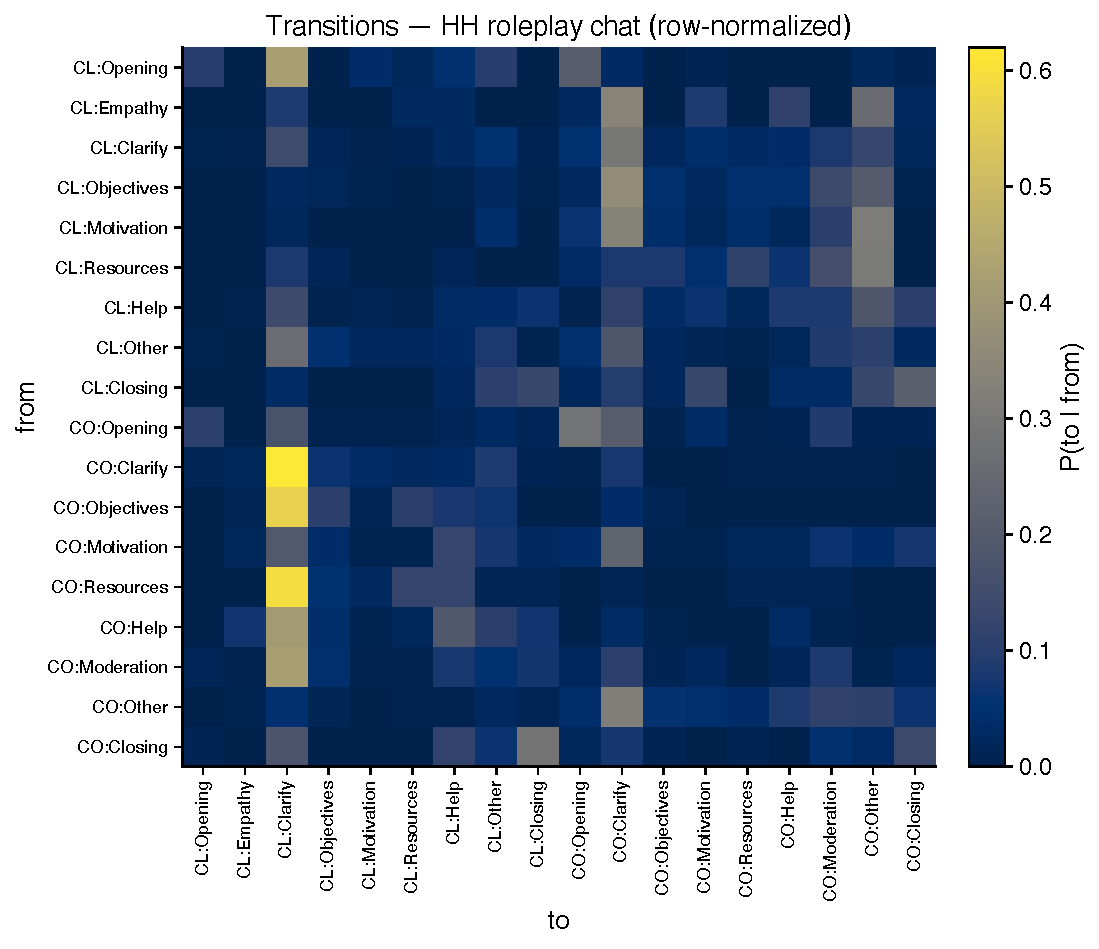
\includegraphics[width=0.68\linewidth]{results/figures/oncoco/transition_HH_roleplay_chat.pdf}
\caption{Transition heatmap for HH roleplay (row-normalized).}
\label{Sfig:transition-hh-chat}
\end{figure}

\begin{figure}[t]
\centering
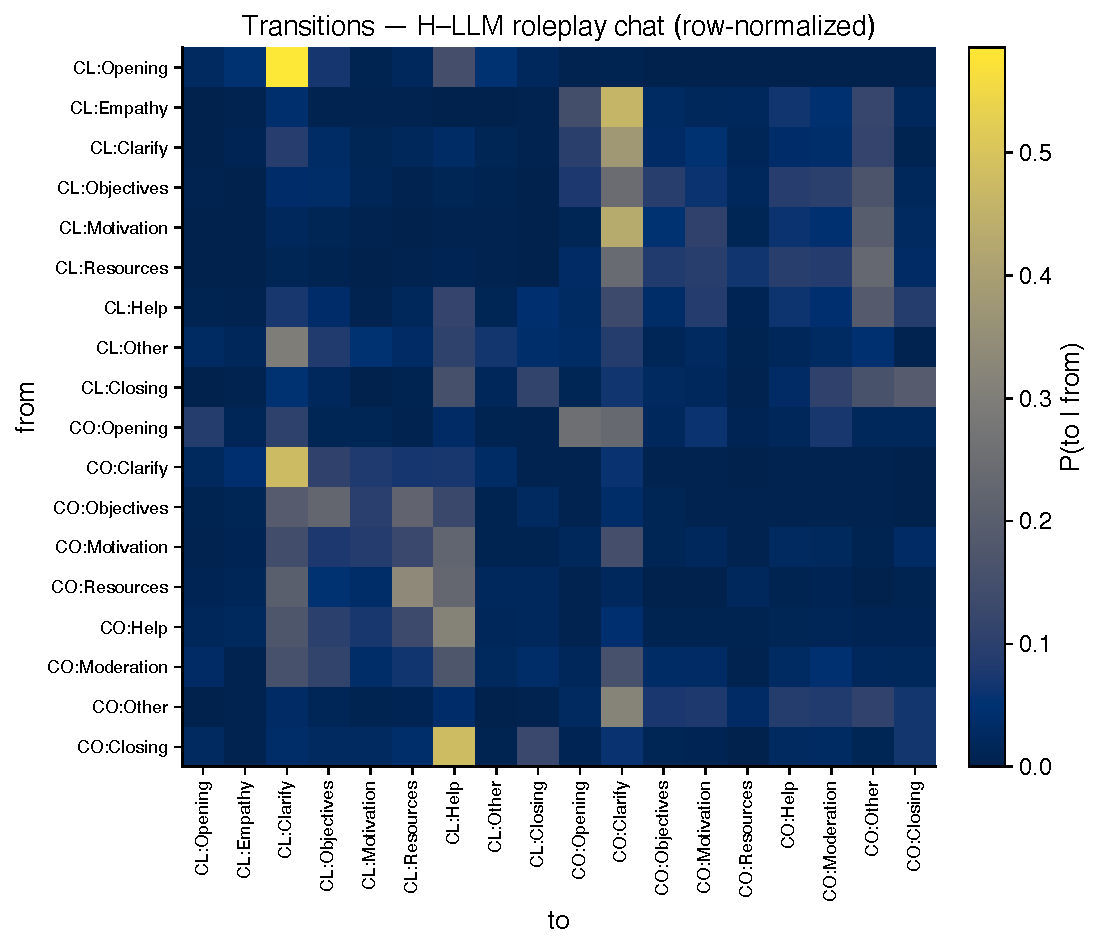
\includegraphics[width=0.68\linewidth]{results/figures/oncoco/transition_H_LLM_roleplay_chat.pdf}
\caption{Transition heatmap for H--LLM roleplay (row-normalized).}
\label{Sfig:transition-hllm-chat}
\end{figure}

\begin{figure}[t]
\centering
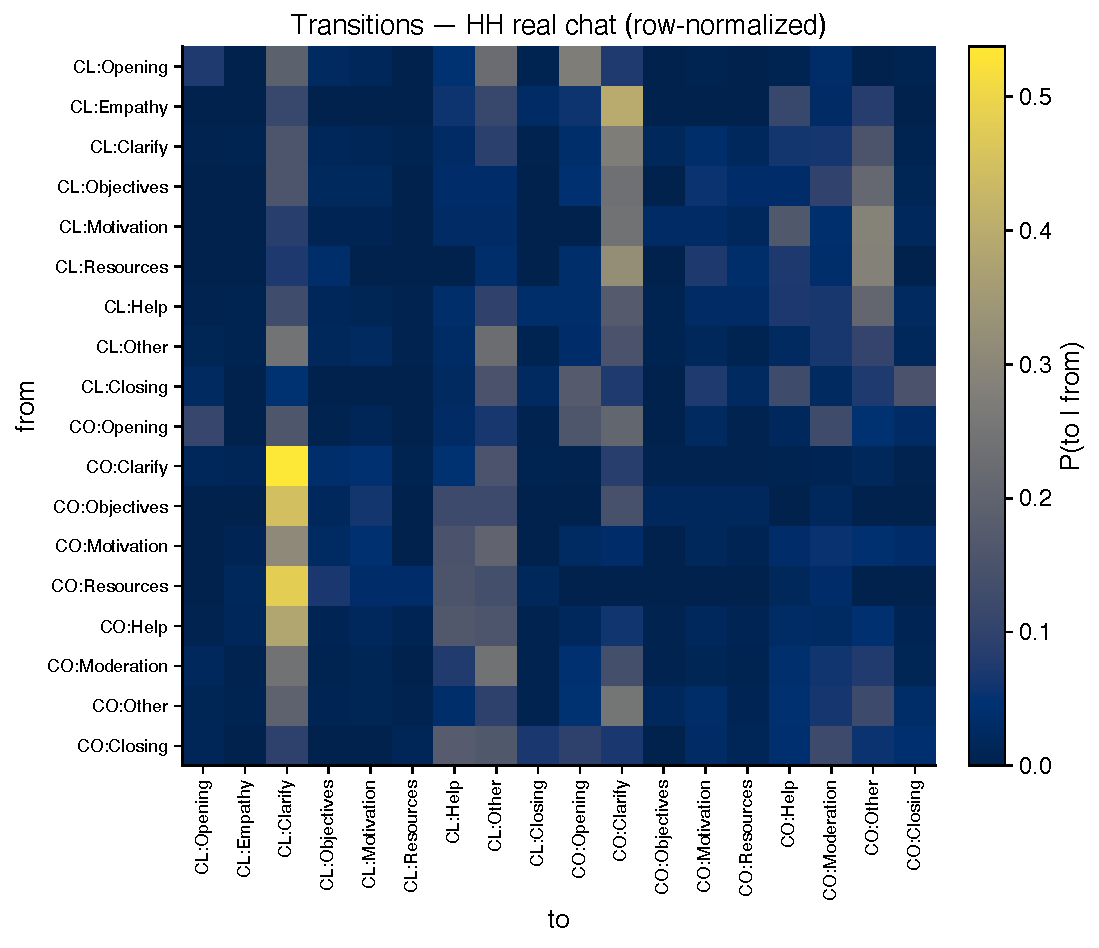
\includegraphics[width=0.68\linewidth]{results/figures/oncoco/transition_HH_real_chat.pdf}
\caption{Transition heatmap for HH real (row-normalized).}
\label{Sfig:transition-hh-real-chat}
\end{figure}

\begin{figure}[t]
\centering
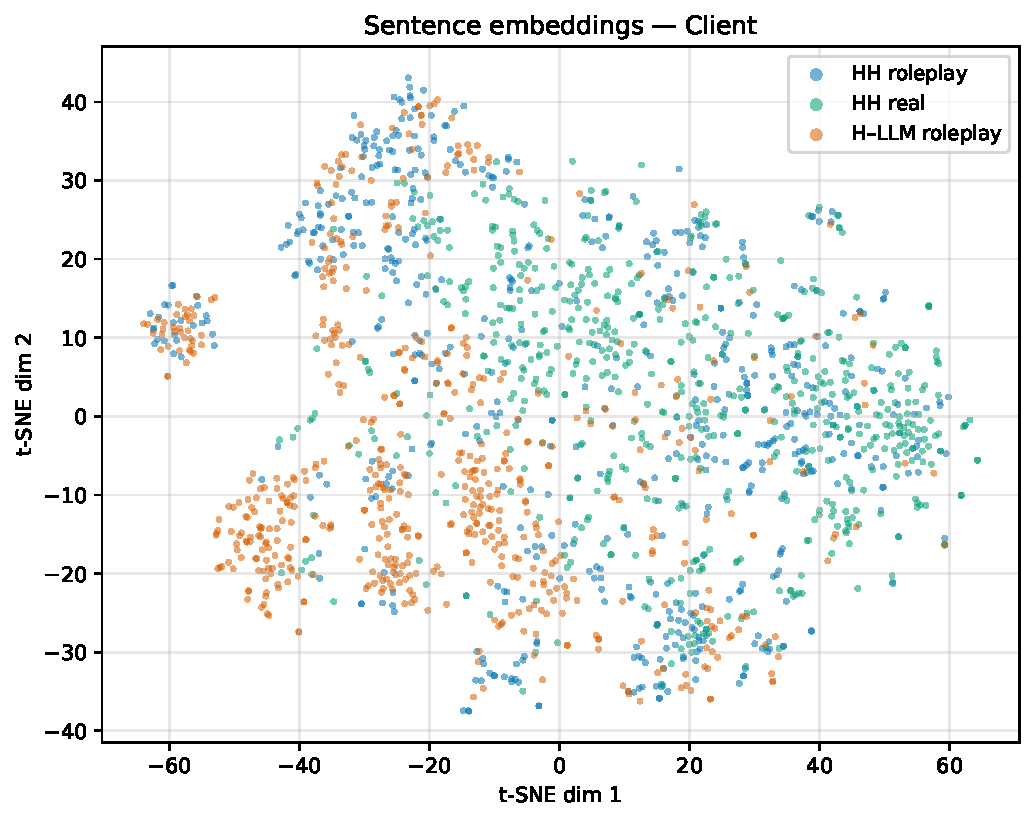
\includegraphics[width=0.70\linewidth]{results/figures/oncoco/tsne_client_chat.pdf}
\caption{t-SNE projection of sentence embeddings by condition (Client).}
\label{Sfig:tsne-client}
\end{figure}

\begin{figure}[t]
\centering
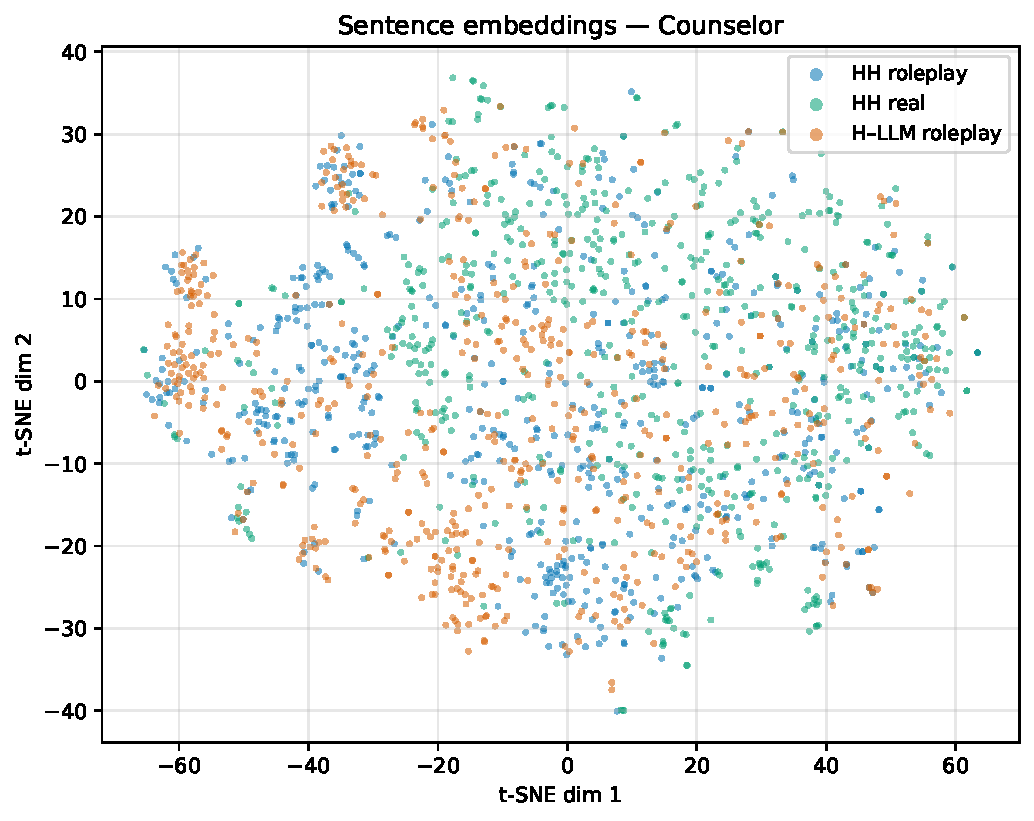
\includegraphics[width=0.70\linewidth]{results/figures/oncoco/tsne_counsellor_chat.pdf}
\caption{t-SNE projection of sentence embeddings by condition (Counselor).}
\label{Sfig:tsne-counselor}
\end{figure}

\begin{figure}[t]
\centering
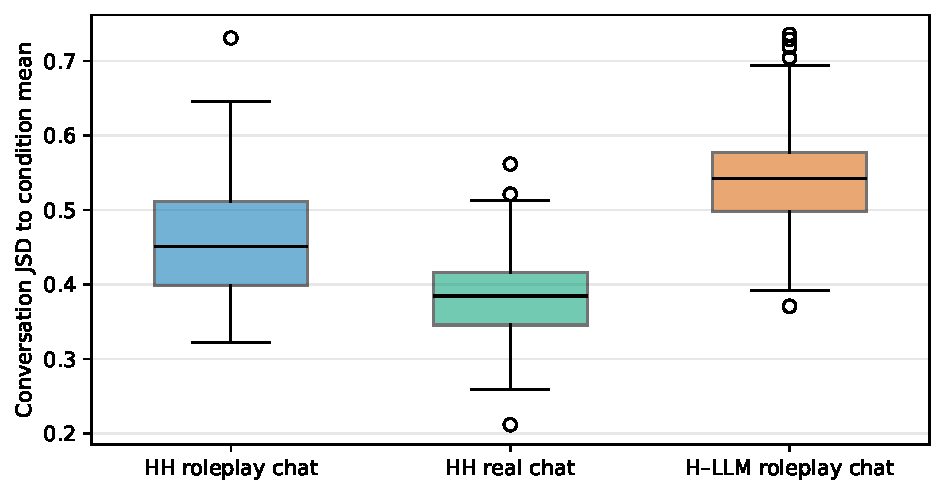
\includegraphics[width=0.72\linewidth]{results/figures/oncoco/within_jsd_client_chat.pdf}
\caption{Within-condition variability (Client): distribution of conversation-level JSD to the condition mean.}
\label{Sfig:within-client}
\end{figure}

\begin{figure}[t]
\centering
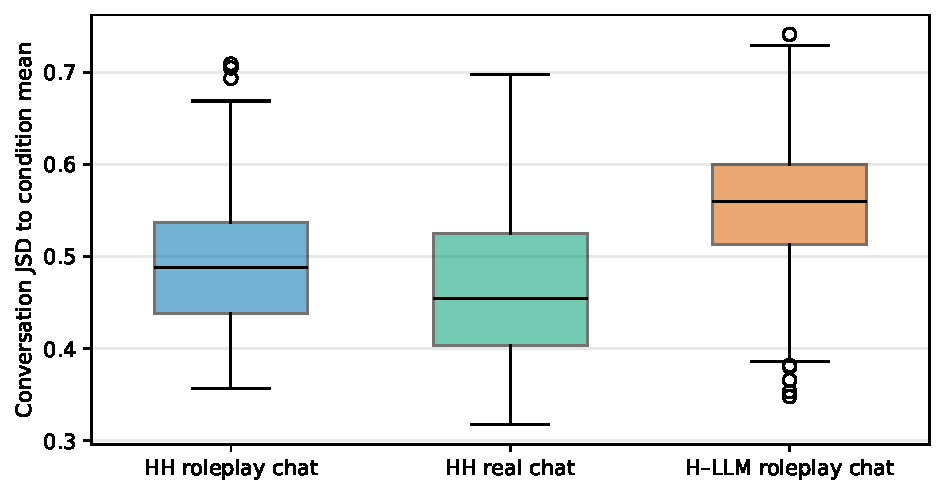
\includegraphics[width=0.72\linewidth]{results/figures/oncoco/within_jsd_counselor_chat.pdf}
\caption{Within-condition variability (Counselor): distribution of conversation-level JSD to the condition mean.}
\label{Sfig:within-counselor}
\end{figure}


\begin{figure}[t]
\centering
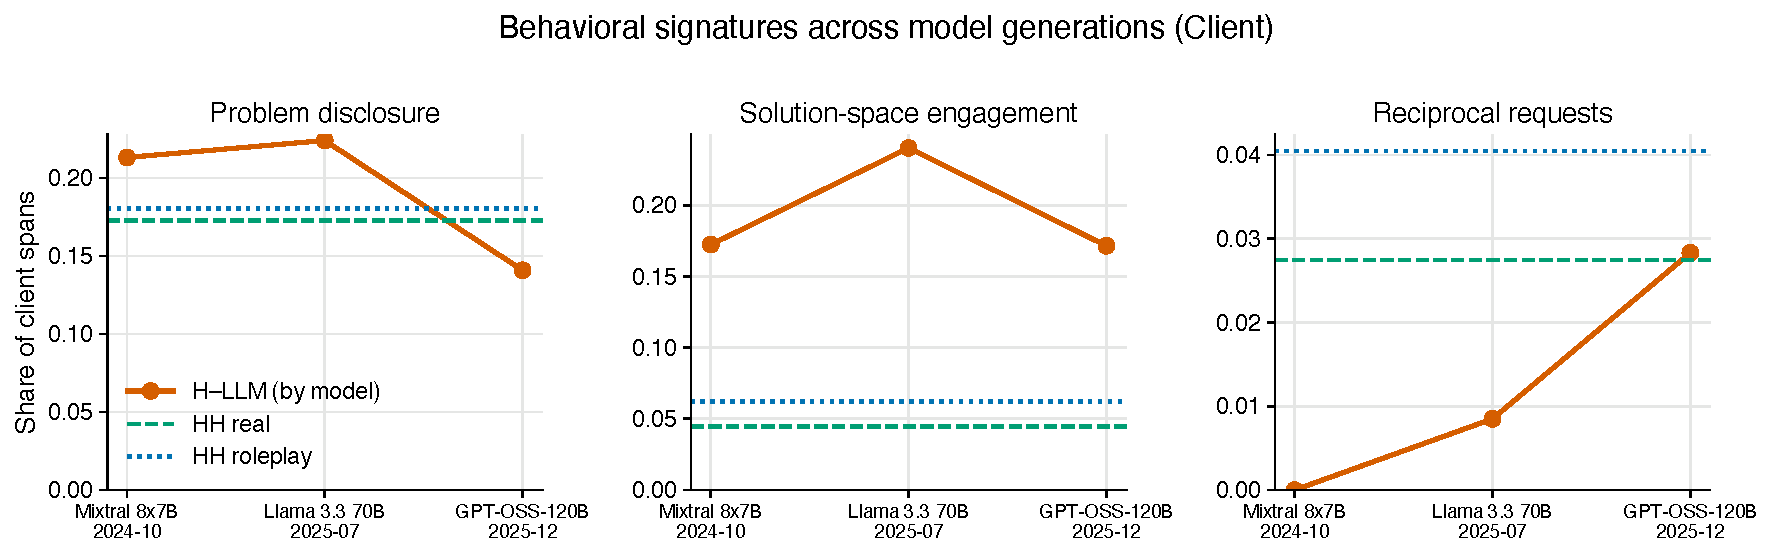
\includegraphics[width=0.85\textwidth]{results/figures/oncoco/behavioral_signatures_evolution.pdf}
\caption{Behavioral signatures across model generations (share of Client spans), with human baselines (dashed for HH real, dotted for HH roleplay). Reciprocal questioning and restraint in problem disclosure improve for the newest model, but solution-space drift persists across generations.}
\label{Sfig:sig-evolution}
\end{figure}


\section{Pre-Declared Category Exclusion Sets}
\label{Ssec:exclusions}
The sensitivity analysis reported in Section~5.5.1 of the main paper removes categories that are arguably fixed by the training setting rather than by counseling behavior. The first two sets below were declared before the analysis was run. S3 is post-hoc and is flagged as such. All three are reproduced here so the choice is auditable.

\textbf{S1: setting-bound (primary).}
\emph{Objective of the assignment} (\texttt{CL-IF-AO-*-Obj-*}) and \emph{Extension of the assignment} (\texttt{CL-IF-AO-*-Ext-*}): the assignment is supplied by the persona prompt and the course task, so a simulated client states it because it is in its context window.
\emph{Definition of counseling objectives} (\texttt{CO-IF-AO-*-ICO-*}): the counselor mirror of the same construct.
\emph{Formalities at the beginning} for both roles (\texttt{CL-FB-*-*-*-*}, \texttt{CO-FA-*-*-*-*}): the opening formalities are platform-dictated. Archived real conversations open with a system join event, and H--LLM sessions open with a scripted first turn.
\emph{Inappropriate remark} for both roles (\texttt{CL-O-*-*-UCO-*}, \texttt{CO-O-*-*-UCO-*}): excluded not as a setting artifact but as a \emph{classifier} artifact. It carries the lowest median confidence of any label with appreciable support (median 0.48--0.60, against 0.88 or above for every category carrying the behavioral signature). The counselor-side code also absorbs 6.5\% of HH real counselor spans against about 1\% in the other two conditions. The client-side code is predicted with higher confidence (0.70--0.78) and is excluded only for symmetry with it. This was established in the confidence diagnostics before the present analysis was run.

\textbf{S2: measurement residual (secondary).} \emph{Other statements} for both roles (\texttt{CL-O-*-*-O-*}, \texttt{CO-O-*-*-O-*}), the residual category for units the classifier cannot place elsewhere. It is kept as a separate tier because it tests a different threat, namely measurement error rather than a setting confound. Merging the two would let one exclusion set carry two arguments.

\textbf{S3: closing formalities (tertiary, reported but not pre-declared).} \emph{Farewell} for both roles (\texttt{CO-FC-*-*-F-*}, \texttt{CL-FC-*-*-F-*}). Session end is partly imposed by the time frame of the exercise, but closing is itself a counseling skill, so the case is weaker and we report rather than assume it.

\textbf{Deliberately not excluded: \emph{Consent}} (\texttt{CL-IF-ACP-*-Cons-*}). It captures brief acknowledgements and agreement rather than a setting artifact. It is the second-largest client-side category and the largest single contributor to the gap. Removing the largest contributor \emph{because} it is large would be the post-hoc selection the objection warns against. It appears instead as one point among all others in the leave-one-out sweep (Figure~\ref{Sfig:loo}), where removing it lowers $\dCL$ by 0.033, from 0.220 to 0.187.

\begin{table}[t]
\caption{Between-condition distance and central gap under each exclusion set, with $k$ the size of the label support after removal and renormalization. Band statistics use HH real's own split-half band recomputed on the reduced support. $\Delta$ carries a 95\% interval from 20{,}000 conversation-level bootstrap resamples, and $^{*}$ marks intervals excluding zero. The ``full'' row reproduces the SaT row of Table~\ref{Stab:unit-ablation}, interval included. Its bounds are taken from that run rather than redrawn here, so the baseline is one number and not two independent estimates of it.}
\label{Stab:category-sensitivity}
\centering
\footnotesize
\setlength{\tabcolsep}{4pt}
\fitwidth{\begin{tabular}{llrrrrc}
\toprule
Exclusion set & Role & $k$ & JSD real--LLM & Band mean & Pctl. & $\Delta$ [95\% CI] \\
\midrule
full & Client & 38 & 0.453 & 0.109 & 100.0 & +0.078$^{*}$ [0.042, 0.109] \\
full & Counselor & 57 & 0.276 & 0.144 & 100.0 & +0.080$^{*}$ [0.042, 0.106] \\
S1 & Client & 33 & 0.460 & 0.108 & 100.0 & +0.067$^{*}$ [0.028, 0.098] \\
S1 & Counselor & 51 & 0.243 & 0.149 & 100.0 & +0.039$^{*}$ [0.001, 0.070] \\
S1+S2 & Client & 32 & 0.391 & 0.122 & 100.0 & +0.008 [-0.029, 0.043] \\
S1+S2 & Counselor & 50 & 0.267 & 0.162 & 100.0 & +0.043$^{*}$ [0.002, 0.077] \\
S1+S2+S3 & Client & 31 & 0.394 & 0.121 & 100.0 & +0.011 [-0.026, 0.046] \\
S1+S2+S3 & Counselor & 48 & 0.270 & 0.161 & 100.0 & +0.044$^{*}$ [0.002, 0.077] \\
\bottomrule
\end{tabular}
}
\end{table}

\begin{figure}[t]
\centering
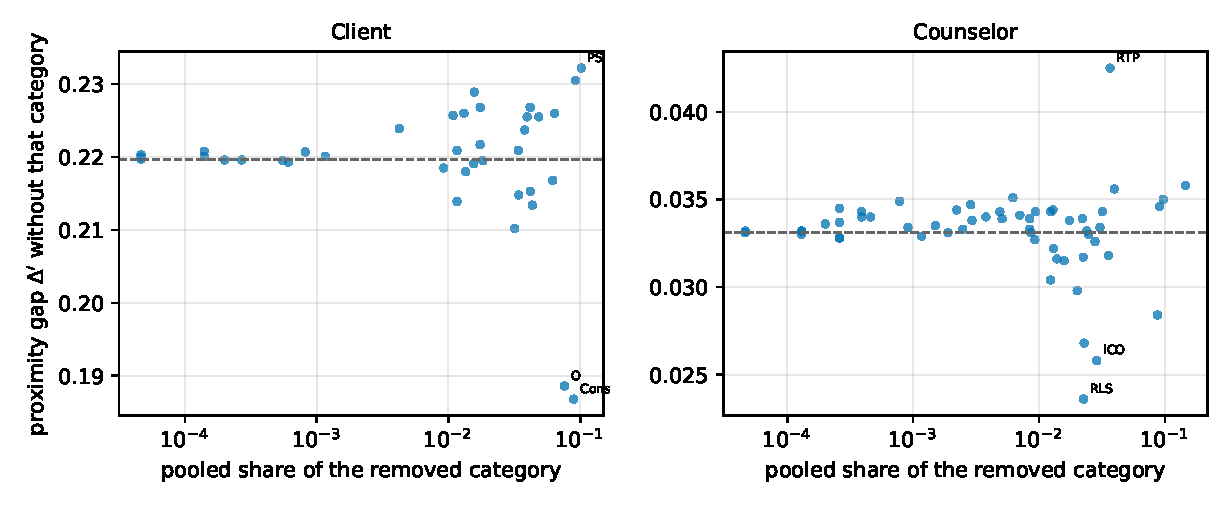
\includegraphics[width=0.92\textwidth]{results/figures/oncoco/leave_one_out_delta.pdf}
\caption{Leave-one-out sweep: the proximity gap $\Delta$ recomputed with each category removed in turn, plotted against that category's pooled share. The dashed line is $\Delta$ on the full support. No single removal brings the client-side $\Delta$ below 0.187. The two categories whose removal lowers it most (\emph{Consent} and \emph{Other statements}) each take off about 0.03.}
\label{Sfig:loo}
\end{figure}

\begin{figure}[t]
\centering
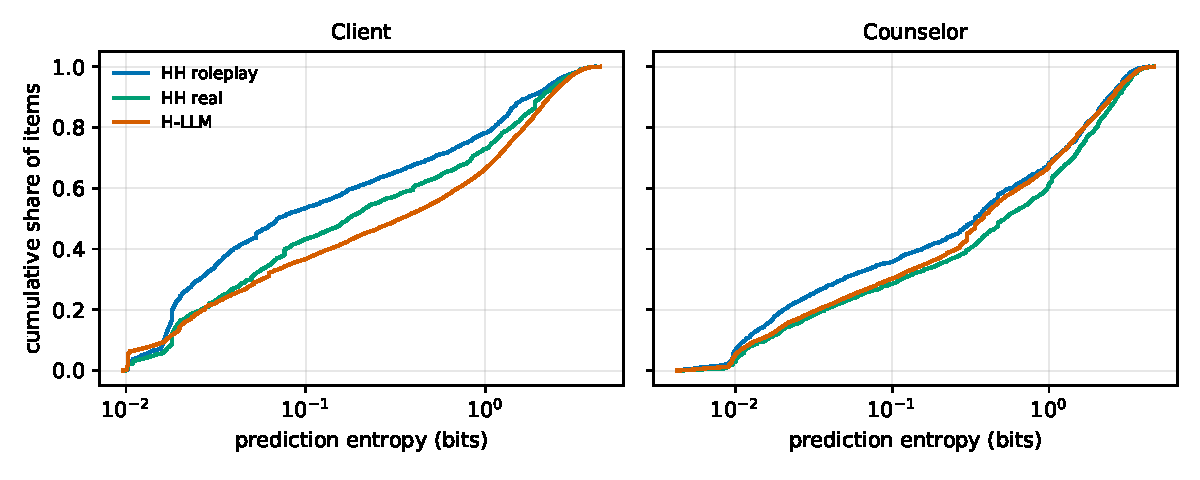
\includegraphics[width=0.80\linewidth]{results/figures/oncoco/confidence_ecdf.pdf}
\caption{Cumulative distribution of prediction entropy by condition and role (symlog $x$-axis). HH real carries the heaviest uncertainty tail on both roles. The pooled client-side confidence ranking in the main text is driven by span length, which the length-matched comparison controls.}
\label{Sfig:confidence-ecdf}
\end{figure}

\section{Methodological Details Referenced from the Main Text}
\label{Ssec:moved}

\textbf{HMM initialisation.} We fit each condition from 20 random initialisations and retain the best-likelihood solution, because the EM likelihood surface for these sequences is strongly multimodal. Across conditions, 20 random initialisations recover 6--11 distinct optima. A single fixed initialisation lands in a markedly inferior one for all three chat conditions (up to $\Delta\log L=1{,}468$), and the resulting states then have near-duplicate output distributions. Table~\ref{Stab:hmm-modelsel} reports the sensitivity sweep over $k=2\ldots8$, in which the cross-validated optimal state count tracks corpus size rather than any property of the conditions.

\textbf{Misspecified segmentation.} The bottom row of Table~\ref{Stab:unit-ablation} is a naive character-class split. It produces 16.2 fragments per message with a mean length of 10 characters, because it splits on a frequent letter rather than only on sentence-final punctuation. The classifier can assign the resulting fragments only to residual categories. Under such a split the between-condition distances collapse by a factor of three to four, the client-side gap shrinks to 0.033, a seventh of its value, and the counselor-side gap changes sign. The row is included in the table so that the contrast with a correctly specified sentence split is visible. It is not a segmentation comparison.

\textbf{Cross-course association (RQ2, secondary).} Across all six courses with unambiguous survey linkage, client-side JSD and disagreement with the realism item correlate at Spearman $\rho$=.83 ($p$=.042). The result is fragile. Two of the six courses contribute only 2 and 9 respondents, and dropping them leaves the direction intact but not the significance ($\rho$=.80, $p$=.20 at $k$=4). A Pearson specification on all six gives $r$=.68 ($p$=.13). We therefore report it as descriptive support for the within-course-line result of Section~5.6 in the main paper rather than as independent evidence.

\begin{table}[t]
\caption{Numbers behind Figure~2 of the main paper: between-condition JSD anchored in the reference condition's split-half noise band (1{,}000 splits), with band mean (noise floor), band P95 (upper edge), the 95th percentile of the size-matched null (nm-P95), and Cram\'er's $V$. All comparisons use HH real as reference.}
\label{Stab:noise-band-chat}
\centering
\footnotesize
\setlength{\tabcolsep}{4pt}
\fitwidth{\begin{tabular}{llrrrrr}
\toprule
Comparison & Role & JSD & Band mean & Band P95 & nm-P95 & $V$ \\
\midrule
HH roleplay & Client & 0.233 & 0.109 & 0.133 & 0.092 & 0.27 \\
HH roleplay & Counselor & 0.242 & 0.143 & 0.168 & 0.116 & 0.27 \\
H--LLM & Client & 0.453 & 0.108 & 0.132 & 0.073 & 0.46 \\
H--LLM & Counselor & 0.276 & 0.143 & 0.168 & 0.091 & 0.26 \\
H--LLM [GPT-OSS-120B] & Client & 0.361 & 0.108 & 0.131 & 0.087 & 0.41 \\
H--LLM [GPT-OSS-120B] & Counselor & 0.293 & 0.143 & 0.167 & 0.111 & 0.33 \\
H--LLM [Llama 3.3 70B] & Client & 0.524 & 0.109 & 0.132 & 0.076 & 0.57 \\
H--LLM [Llama 3.3 70B] & Counselor & 0.298 & 0.144 & 0.169 & 0.098 & 0.30 \\
H--LLM [Mixtral 8x7B] & Client & 0.495 & 0.109 & 0.132 & 0.086 & 0.54 \\
H--LLM [Mixtral 8x7B] & Counselor & 0.292 & 0.144 & 0.170 & 0.110 & 0.33 \\
\bottomrule
\end{tabular}
}
\end{table}

\begin{table}[t]
\caption{Distributional proximity to HH real by model with 95\% conversation-level bootstrap CIs (lower = closer). These are the intervals drawn in the per-model rows of Figure~2 of the main paper.}
\label{Stab:model-realness}
\centering
\footnotesize
\setlength{\tabcolsep}{3pt}
\fitwidth{\begin{tabular}{lcc}
\toprule
Model & Client JSD [95\% CI] & Counselor JSD [95\% CI] \\
\midrule
GPT-OSS-120B & 0.361 [0.338, 0.402] & 0.293 [0.274, 0.338] \\
Llama 3.3 70B & 0.524 [0.503, 0.552] & 0.298 [0.286, 0.332] \\
Mixtral 8x7B & 0.495 [0.468, 0.530] & 0.292 [0.272, 0.338] \\
\bottomrule
\end{tabular}
}
\end{table}

\begin{table}[t]
\caption{Sequential structure summary (role-aware transitions) for the three chat conditions. All three are dominated by cross-role alternation. Section~5.3 of the main paper reads these differences.}
\label{Stab:transition-summary}
\centering
\footnotesize
\setlength{\tabcolsep}{3pt}
\fitwidth{\begin{tabular}{lccc}
\toprule
Condition & Same-role & Cross-role & Self-transition \\
\midrule
HH roleplay & 0.323 & 0.677 & 0.101 \\
HH real & 0.365 & 0.635 & 0.115 \\
H--LLM roleplay & 0.292 & 0.708 & 0.070 \\
\bottomrule
\end{tabular}
}
\end{table}

\begin{table}[t]
\caption{All 70 transition cells that shift significantly for H--LLM vs HH real under FDR control at $q=0.10$, sorted by absolute shift and set in two column blocks. Rates are row-normalized transition probabilities in each condition. $\Delta$ is the H--LLM rate minus the HH real rate, $n$ the combined transition count, and $p$ the empirical $p$-value from 2{,}000 split-half resamples of HH real. The smallest attainable value is shown as $<$0.001. Section~5.3 of the main paper reports the counts and the largest shifts.}
\label{Stab:transition-fdr-hllm}
\centering
\footnotesize
\setlength{\tabcolsep}{3pt}
\fitwidth{\begin{tabular}{llrrrrr@{\hspace{1.5em}}llrrrrr}
\toprule
From & To & H--LLM & HH real & $\Delta$ & $n$ & $p$ & From & To & H--LLM & HH real & $\Delta$ & $n$ & $p$ \\
\midrule
CL:Opening & CL:Clarify & 0.585 & 0.192 & $+0.394$ & 441 & $<$0.001 & CL:Clarify & CO:Opening & 0.100 & 0.036 & $+0.064$ & 421 & $<$0.001 \\
CO:Closing & CL:Help & 0.480 & 0.178 & $+0.302$ & 260 & 0.002 & CO:Clarify & CL:Resources & 0.070 & 0.008 & $+0.062$ & 292 & $<$0.001 \\
CO:Resources & CL:Resources & 0.337 & 0.035 & $+0.302$ & 97 & $<$0.001 & CL:Help & CO:Motivation & 0.087 & 0.029 & $+0.058$ & 156 & 0.004 \\
CL:Opening & CO:Opening & 0.004 & 0.275 & $-0.271$ & 36 & $<$0.001 & CL:Other & CO:Other & 0.048 & 0.106 & $-0.058$ & 84 & 0.011 \\
CO:Objectives & CL:Resources & 0.221 & 0.000 & $+0.221$ & 146 & $<$0.001 & CO:Other & CO:Objectives & 0.075 & 0.020 & $+0.055$ & 136 & $<$0.001 \\
CO:Moderation & CL:Other & 0.025 & 0.243 & $-0.218$ & 85 & $<$0.001 & CL:Opening & CL:Empathy & 0.055 & 0.000 & $+0.055$ & 39 & $<$0.001 \\
CO:Help & CL:Clarify & 0.175 & 0.384 & $-0.209$ & 214 & $<$0.001 & CO:Help & CL:Motivation & 0.072 & 0.020 & $+0.052$ & 61 & 0.004 \\
CO:Objectives & CL:Objectives & 0.227 & 0.020 & $+0.206$ & 151 & $<$0.001 & CO:Other & CO:Help & 0.091 & 0.042 & $+0.049$ & 174 & 0.003 \\
CO:Motivation & CL:Other & 0.009 & 0.203 & $-0.194$ & 31 & 0.021 & CO:Other & CO:Motivation & 0.079 & 0.032 & $+0.047$ & 149 & 0.002 \\
CL:Opening & CL:Other & 0.052 & 0.225 & $-0.173$ & 64 & 0.018 & CO:Clarify & CL:Motivation & 0.081 & 0.044 & $+0.037$ & 368 & 0.015 \\
CO:Other & CL:Clarify & 0.031 & 0.197 & $-0.165$ & 151 & $<$0.001 & CO:Other & CO:Closing & 0.068 & 0.032 & $+0.036$ & 131 & 0.004 \\
CO:Help & CL:Help & 0.318 & 0.167 & $+0.151$ & 284 & 0.001 & CL:Other & CL:Closing & 0.040 & 0.006 & $+0.034$ & 18 & $<$0.001 \\
CO:Help & CL:Other & 0.017 & 0.157 & $-0.140$ & 44 & 0.013 & CO:Clarify & CL:Empathy & 0.045 & 0.013 & $+0.033$ & 196 & $<$0.001 \\
CL:Closing & CL:Help & 0.153 & 0.025 & $+0.129$ & 36 & $<$0.001 & CO:Moderation & CL:Closing & 0.036 & 0.004 & $+0.032$ & 31 & $<$0.001 \\
CO:Motivation & CL:Resources & 0.127 & 0.000 & $+0.127$ & 112 & $<$0.001 & CL:Other & CL:Motivation & 0.054 & 0.024 & $+0.030$ & 34 & 0.012 \\
CO:Help & CL:Resources & 0.134 & 0.010 & $+0.124$ & 108 & $<$0.001 & CL:Resources & CO:Closing & 0.030 & 0.000 & $+0.030$ & 29 & $<$0.001 \\
CO:Clarify & CL:Other & 0.033 & 0.153 & $-0.120$ & 266 & $<$0.001 & CO:Moderation & CO:Objectives & 0.033 & 0.004 & $+0.029$ & 29 & $<$0.001 \\
CO:Motivation & CO:Clarify & 0.152 & 0.035 & $+0.117$ & 138 & $<$0.001 & CL:Empathy & CO:Objectives & 0.028 & 0.000 & $+0.028$ & 10 & $<$0.001 \\
CL:Clarify & CO:Clarify & 0.379 & 0.273 & $+0.106$ & 1776 & 0.009 & CO:Objectives & CL:Closing & 0.027 & 0.000 & $+0.027$ & 18 & $<$0.001 \\
CO:Moderation & CL:Objectives & 0.113 & 0.008 & $+0.105$ & 97 & $<$0.001 & CL:Other & CL:Resources & 0.031 & 0.005 & $+0.027$ & 14 & $<$0.001 \\
CL:Opening & CL:Help & 0.151 & 0.050 & $+0.101$ & 114 & 0.008 & CL:Help & CO:Objectives & 0.035 & 0.008 & $+0.026$ & 61 & $<$0.001 \\
CO:Moderation & CL:Help & 0.174 & 0.076 & $+0.098$ & 166 & 0.002 & CO:Closing & CL:Objectives & 0.025 & 0.000 & $+0.025$ & 13 & $<$0.001 \\
CO:Other & CL:Other & 0.001 & 0.096 & $-0.095$ & 50 & 0.003 & CO:Closing & CL:Motivation & 0.025 & 0.000 & $+0.025$ & 13 & $<$0.001 \\
CL:Objectives & CO:Objectives & 0.095 & 0.000 & $+0.095$ & 115 & $<$0.001 & CO:Moderation & CL:Motivation & 0.036 & 0.011 & $+0.024$ & 33 & 0.008 \\
CO:Help & CL:Objectives & 0.101 & 0.010 & $+0.091$ & 82 & $<$0.001 & CO:Opening & CO:Objectives & 0.023 & 0.000 & $+0.023$ & 22 & $<$0.001 \\
CL:Help & CL:Other & 0.012 & 0.100 & $-0.088$ & 45 & 0.024 & CO:Other & CO:Resources & 0.031 & 0.010 & $+0.021$ & 58 & 0.018 \\
CL:Closing & CO:Moderation & 0.110 & 0.025 & $+0.085$ & 26 & $<$0.001 & CL:Opening & CL:Resources & 0.021 & 0.000 & $+0.021$ & 15 & $<$0.001 \\
CL:Resources & CO:Objectives & 0.083 & 0.000 & $+0.083$ & 81 & $<$0.001 & CL:Clarify & CL:Objectives & 0.034 & 0.015 & $+0.019$ & 147 & 0.019 \\
CL:Clarify & CL:Other & 0.013 & 0.093 & $-0.079$ & 168 & $<$0.001 & CL:Other & CL:Opening & 0.029 & 0.011 & $+0.017$ & 17 & 0.028 \\
CL:Motivation & CO:Motivation & 0.108 & 0.029 & $+0.079$ & 78 & 0.002 & CO:Help & CL:Closing & 0.021 & 0.005 & $+0.017$ & 18 & $<$0.001 \\
CL:Other & CL:Help & 0.105 & 0.030 & $+0.075$ & 56 & $<$0.001 & CO:Opening & CL:Empathy & 0.015 & 0.000 & $+0.015$ & 15 & $<$0.001 \\
CO:Clarify & CL:Objectives & 0.108 & 0.037 & $+0.071$ & 470 & $<$0.001 & CL:Help & CL:Resources & 0.019 & 0.004 & $+0.015$ & 33 & $<$0.001 \\
CL:Help & CO:Closing & 0.091 & 0.025 & $+0.066$ & 162 & $<$0.001 & CO:Motivation & CO:Objectives & 0.013 & 0.000 & $+0.013$ & 11 & $<$0.001 \\
CL:Other & CL:Objectives & 0.083 & 0.018 & $+0.065$ & 40 & $<$0.001 & CL:Clarify & CL:Resources & 0.020 & 0.008 & $+0.012$ & 85 & 0.012 \\
CO:Moderation & CL:Resources & 0.064 & 0.000 & $+0.064$ & 54 & $<$0.001 & CL:Resources & CL:Help & 0.010 & 0.000 & $+0.010$ & 10 & $<$0.001 \\
\bottomrule
\end{tabular}
}
\end{table}

\begin{table}[t]
\caption{All 20 transition cells that shift significantly for HH roleplay vs HH real under FDR control at $q=0.10$, sorted by absolute shift. Columns as in Table~\ref{Stab:transition-fdr-hllm}.}
\label{Stab:transition-fdr-roleplay}
\centering
\footnotesize
\setlength{\tabcolsep}{3pt}
\fitwidth{\begin{tabular}{llrrrrr}
\toprule
From & To & HH roleplay & HH real & $\Delta$ & $n$ & $p$ \\
\midrule
CL:Opening & CL:Clarify & 0.422 & 0.192 & $+0.230$ & 66 & $<$0.001 \\
CO:Closing & CL:Closing & 0.287 & 0.069 & $+0.219$ & 32 & $<$0.001 \\
CO:Motivation & CO:Clarify & 0.232 & 0.035 & $+0.196$ & 29 & $<$0.001 \\
CO:Moderation & CL:Other & 0.056 & 0.243 & $-0.187$ & 78 & 0.001 \\
CO:Moderation & CL:Clarify & 0.422 & 0.243 & $+0.178$ & 169 & $<$0.001 \\
CO:Other & CL:Clarify & 0.051 & 0.197 & $-0.146$ & 114 & 0.001 \\
CL:Resources & CO:Moderation & 0.161 & 0.036 & $+0.126$ & 11 & 0.001 \\
CO:Resources & CL:Resources & 0.122 & 0.035 & $+0.087$ & 11 & 0.011 \\
CL:Help & CO:Closing & 0.103 & 0.025 & $+0.078$ & 22 & $<$0.001 \\
CO:Moderation & CL:Closing & 0.072 & 0.004 & $+0.069$ & 19 & $<$0.001 \\
CO:Help & CL:Empathy & 0.070 & 0.015 & $+0.054$ & 11 & $<$0.001 \\
CO:Other & CO:Help & 0.085 & 0.042 & $+0.043$ & 48 & 0.007 \\
CO:Other & CO:Objectives & 0.060 & 0.020 & $+0.040$ & 29 & 0.003 \\
CL:Clarify & CL:Other & 0.054 & 0.093 & $-0.039$ & 175 & 0.016 \\
CO:Moderation & CL:Objectives & 0.044 & 0.008 & $+0.037$ & 13 & $<$0.001 \\
CL:Other & CL:Objectives & 0.049 & 0.018 & $+0.032$ & 22 & 0.001 \\
CO:Other & CO:Closing & 0.063 & 0.032 & $+0.031$ & 36 & 0.013 \\
CO:Other & CO:Resources & 0.038 & 0.010 & $+0.028$ & 17 & $<$0.001 \\
CO:Clarify & CL:Resources & 0.025 & 0.008 & $+0.017$ & 25 & 0.009 \\
CL:Clarify & CO:Closing & 0.021 & 0.008 & $+0.013$ & 32 & 0.008 \\
\bottomrule
\end{tabular}
}
\end{table}

\begin{table}[t]
\caption{Message length and surface register of client messages per condition and, within H--LLM, per model, persona brevity cue, and template family (Section~5.2 of the main paper). Median words per client message with interquartile range, and the share of messages without sentence-final punctuation. ``Llama x template\_family'' restricts the template contrast to the one model that ran under both families.}
\label{Stab:verbosity}
\centering
\footnotesize
\setlength{\tabcolsep}{4pt}
\fitwidth{\begin{tabular}{llrrrr}
\toprule
Grouping & Level & Conv. & Client msgs & Median words [IQR] & No final punct. \\
\midrule
condition & HH roleplay & 68 & 1366 & 12 [5, 26] & 38.7\% \\
 & HH real & 53 & 1632 & 10 [3, 21] & 85.4\% \\
 & H--LLM & 414 & 7758 & 39 [28, 51] & 9.2\% \\
model & Mixtral 8x7B & 86 & 1464 & 30 [22, 39] & 0.0\% \\
 & Llama 3.3 70B & 238 & 4804 & 44 [35, 57] & 0.3\% \\
 & GPT-OSS-120B & 90 & 1490 & 25 [17, 37] & 47.1\% \\
brevity\_persona & yes & 225 & 4312 & 32 [23, 40] & 16.5\% \\
 & no & 189 & 3446 & 50 [39, 63] & 0.1\% \\
template\_family & plain & 207 & 3330 & 45 [26, 63] & 21.5\% \\
 & chat & 121 & 2964 & 39 [33, 47] & 0.0\% \\
 & not logged & 86 & 1464 & 30 [22, 39] & 0.0\% \\
Llama x template\_family & plain & 117 & 1840 & 59 [47, 72] & 0.8\% \\
 & chat & 121 & 2964 & 39 [33, 47] & 0.0\% \\
\bottomrule
\end{tabular}
}
\end{table}

\begin{table}[t]
\caption{Client-side distance to HH real and proximity gap $\Delta$ per prompt configuration, SaT spans, with 95\% intervals from 20{,}000 conversation-level bootstrap resamples (Section~5.4 of the main paper). Template family is nested in model and semester: GPT-OSS-120B ran plain templates only and Mixtral 8x7B logged no prompts. The persona-matched block restricts Llama 3.3 70B to the four personas that appear under both families. The difference between its two rows is 0.164 [0.129, 0.194].}
\label{Stab:prompt-variants}
\centering
\footnotesize
\setlength{\tabcolsep}{4pt}
\fitwidth{\begin{tabular}{llrrcc}
\toprule
Block & Prompt configuration & Conv. & Med. words & JSD real--LLM [95\% CI] & $\Delta$ [95\% CI] \\
\midrule
all & all H--LLM & 414 & 38 & 0.453 [0.429, 0.483] & +0.220$^{*}$ [0.178, 0.243] \\
\addlinespace
template family & plain template & 207 & 52 & 0.396 [0.372, 0.430] & +0.163$^{*}$ [0.122, 0.190] \\
 & chat template & 121 & 39 & 0.597 [0.575, 0.625] & +0.364$^{*}$ [0.322, 0.387] \\
 & prompt not logged & 86 & 30 & 0.495 [0.469, 0.529] & +0.262$^{*}$ [0.220, 0.289] \\
\addlinespace
persona brevity cue & persona asks for brevity & 225 & 30 & 0.448 [0.422, 0.482] & +0.215$^{*}$ [0.171, 0.242] \\
 & persona silent on length & 189 & 54 & 0.487 [0.464, 0.517] & +0.254$^{*}$ [0.213, 0.278] \\
\addlinespace
model x template family & Mixtral 8x7B, not logged & 86 & 30 & 0.495 [0.469, 0.529] & +0.262$^{*}$ [0.220, 0.289] \\
\addlinespace
model x persona brevity cue & Mixtral 8x7B, brevity yes & 83 & 30 & 0.497 [0.471, 0.531] & +0.264$^{*}$ [0.221, 0.291] \\
\addlinespace
model x template family & Llama 3.3 70B, plain & 117 & 61 & 0.492 [0.471, 0.521] & +0.259$^{*}$ [0.218, 0.283] \\
 & Llama 3.3 70B, chat & 121 & 39 & 0.597 [0.575, 0.625] & +0.364$^{*}$ [0.322, 0.387] \\
\addlinespace
model x persona brevity cue & Llama 3.3 70B, brevity yes & 70 & 36 & 0.600 [0.576, 0.633] & +0.367$^{*}$ [0.324, 0.395] \\
 & Llama 3.3 70B, brevity no & 168 & 56 & 0.507 [0.485, 0.536] & +0.275$^{*}$ [0.233, 0.299] \\
\addlinespace
model x template family & GPT-OSS-120B, plain & 90 & 26 & 0.361 [0.336, 0.400] & +0.128$^{*}$ [0.085, 0.161] \\
\addlinespace
model x persona brevity cue & GPT-OSS-120B, brevity yes & 72 & 26 & 0.362 [0.335, 0.405] & +0.129$^{*}$ [0.083, 0.165] \\
 & GPT-OSS-120B, brevity no & 18 & 29 & 0.434 [0.414, 0.496] & +0.201$^{*}$ [0.165, 0.255] \\
\addlinespace
Llama, persona-matched & Llama 3.3 70B, plain, persona-matched & 45 & 64 & 0.491 [0.466, 0.528] & +0.258$^{*}$ [0.215, 0.289] \\
 & Llama 3.3 70B, chat, persona-matched & 36 & 38 & 0.655 [0.632, 0.686] & +0.422$^{*}$ [0.379, 0.449] \\
\bottomrule
\end{tabular}
}
\end{table}

\begin{table}[t]
\caption{Size-matched subsample check (Section~5.5.3 of the main paper). Client-side $\Delta$ recomputed on 1{,}000 random draws of 68 H--LLM conversations without replacement, the size of the HH roleplay condition, pooled and within each model. Columns give the mean, the central 95\% range of the draws, and the share of draws above zero.}
\label{Stab:sizematched}
\centering
\footnotesize
\setlength{\tabcolsep}{4pt}
\fitwidth{\begin{tabular}{lrrcr}
\toprule
Pool & Conv. in pool & Mean $\Delta$ & [P2.5, P97.5] & Share $>0$ \\
\midrule
all H--LLM & 414 & +0.225 & [0.194, 0.256] & 100.0\% \\
Mixtral 8x7B & 86 & +0.263 & [0.254, 0.272] & 100.0\% \\
Llama 3.3 70B & 238 & +0.294 & [0.272, 0.316] & 100.0\% \\
GPT-OSS-120B & 90 & +0.130 & [0.116, 0.144] & 100.0\% \\
\bottomrule
\end{tabular}
}
\end{table}

\begin{table}[t]
\caption{The central RQ1 gap across units of analysis (Section~5.5 of the main paper).
Columns give the client- and counselor-side distances from HH real to H--LLM roleplay and to HH roleplay, and their difference ($\dCL$ and $\dCO$), with a 95\% interval from 20{,}000 conversation-level resamples. $^{*}$ marks a gap whose whole interval lies above zero.
The bottom row is a misspecified character-class split, not a real segmentation.}
\label{Stab:unit-ablation}
\centering
\footnotesize
\setlength{\tabcolsep}{4pt}
\fitwidth{\begin{tabular}{lcccccc}
\toprule
 & \multicolumn{3}{c}{Client} & \multicolumn{3}{c}{Counselor} \\
\cmidrule(lr){2-4}\cmidrule(lr){5-7}
Unit of analysis & real--LLM & real--roleplay & $\Delta$ [95\% CI] & real--LLM & real--roleplay & $\Delta$ [95\% CI] \\
\midrule
SaT spans & 0.453 & 0.233 & +0.220$^{*}$ [0.178, 0.243] & 0.276 & 0.242 & +0.033$^{*}$ [0.000, 0.049] \\
Regex spans & 0.342 & 0.222 & +0.120$^{*}$ [0.086, 0.143] & 0.245 & 0.225 & +0.020 [-0.012, 0.041] \\
Messages & 0.475 & 0.242 & +0.233$^{*}$ [0.182, 0.258] & 0.320 & 0.298 & +0.022 [-0.022, 0.047] \\
\midrule
Naive character split & 0.106 & 0.073 & +0.033$^{*}$ [0.011, 0.048] & 0.073 & 0.093 & -0.019$^{*}$ [-0.030, -0.010] \\
\bottomrule
\end{tabular}
}
\end{table}

\section{Prompt-Replay Experiment}
\label{Ssec:replay}
This section documents the replay experiment of Section~5.7 in the main paper. Its code and prompts are in the companion repository (directories \texttt{analysis/prompt\_replay/} and \texttt{prompts/replay/}). The generated client turns are not released, because the requests carry the unmasked counselor turns of the original conversations.

\textbf{Design.} The platform logged, for every simulated-client turn, the complete prompt it sent to the model, including the persona profile and the conversation history up to that turn. Each turn can therefore be generated again as an independent request whose context is the original history. We regenerate all 1{,}489 client turns of the 90 GPT-OSS-120B conversations (one turn has no logged prompt and is skipped) with the same model (\texttt{openai/gpt-oss-120b}, served with vLLM 0.28 on one A100 80\,GB) and the platform's sampling settings (temperature 1, at most 3{,}000 tokens, no penalties). The prompt is sent as one user message. Only the instruction block of the prompt varies between arms. The persona block and the history block are byte-identical across arms, which the request builder asserts for every turn. The counselor turns are the original human turns in every arm. This isolates the prompt effect and leaves the counselor's reaction to a changed client untested.

\textbf{Arms.} Arm O passes the original client text through the current pipeline and is the comparison base. Arm A resends the logged prompt unchanged and tests whether our setup reproduces the deployment. Arm B replaces the instruction block by a generic cue (``write like a real help-seeking person in a counseling chat, realistic, authentic, short''). Arm C replaces it by five rules written against the five signatures of Section~5.2 in the main paper: disclose only what the counselor asked for and at most one new aspect per message, stay with the problem when the counselor proposes something and reject what does not fit, ask the counselor a question in about every third message, do not thank or confirm, and write at most 20 words in chat register without a final period. Arm D keeps C and doses the two rules that overshot: questions become rare (``at most once or twice in the whole conversation''), and short assent is allowed while thanking in every message is not. Arm E keeps D and allows positive feedback about as often as disagreement. Arm F decodes the history before each turn with the HH real phase model of Section~5.3 in the main paper and uses one rule block for the clarification phase (as D, with entry into the help phase left to the counselor) and one for the help phase (feedback on suggestions allowed, no new problem, no planning, closing accepted). Arm G keeps F, removes the form examples from the help-phase block, forbids commitments to implementation (``whether it helps, yes, what you will do with it, no''), and phrases entry into the help phase conditionally instead of ``once''.

\textbf{Measurement.} Every arm is converted to the chat format of the corpus and classified with the unchanged pipeline (SaT-6l with the OnCoCo adapter, XLM-RoBERTa-large OnCoCo classifier). The counselor spans are identical across arms, which we verify. The current segmentation reproduces the paper corpus exactly for about 90\% of messages, with differences concentrated on emoji and special characters, so arm O and not the paper's deployment row is the comparison base. The differing messages are split more finely, 1.87 spans per client message in arm O against 1.68 in the deployment, with more one-word spans (14.7\% against 12.1\%) and more \emph{Other statements} (10.3\% against 7.0\%). On whole messages, where no segmentation is involved, arm O and the deployment are indistinguishable (JSD 0.003), and on spans arm O lies at 0.058 from the deployment row, inside the deployment's own split-half band (95th percentile 0.158). Arm A, the logged prompt replayed, lies at 0.083 from the deployment row, also inside that band. All arms pass through the same current segmentation, so differences between arms are not segmentation effects. Table~\ref{Stab:replay-all} gives every arm on the span and the message unit. Figure~\ref{Sfig:replay-deciles} gives the decile profiles.

\textbf{Profiles.} Equal distance to HH real does not mean equal behavior. Arms D and G lie 0.233 and 0.213 from HH real but 0.322 and 0.302 from HH roleplay, farther than either lies from real counseling. Arm D matches real clients on the residual \emph{Other statements} (0.232 against 0.241) and on \emph{Consent} (0.182 against 0.171), where role-play clients depart (0.108 and 0.223). It departs where role-play clients do not, with almost no \emph{General positive feedback} (0.004 against 0.047 in HH real and 0.046 in HH roleplay) and few \emph{General requests} (0.007 against 0.027 and 0.040). The dosed arms therefore reach the distance of a human role-play partner by a different route.

\textbf{Phases.} The three-state HMM fitted on HH real (Section~5.3 in the main paper) separates an opening phase (6\% of spans), a clarification phase (80\%), and a help-and-closing phase (15\%). Every condition is decoded with this one reference model, because states of separately fitted models are not comparable: the third state of the H--LLM fit is a solution-planning mode (Help 0.27, Resources 0.10, Objectives 0.11) that occupies 39\% of its spans, while the third state of HH real is a help-and-closing phase. Under the reference model, real clients express problems, questions, and disagreement in the clarification phase and positive feedback almost only in the help phase (0.241 of their spans there against 0.026 in clarification). Real clients initiate 44\% of the moves from clarification into help. The turn-level test decodes the original history before each client turn and again with the client's spans appended. A move from clarification to help counts as client-led entry. Table~\ref{Stab:phase-transitions} reports the rates.

\textbf{Example echo.} Arm F copied the form examples of its help-phase block. 105 of its 243 help-phase turns read ``ja das hilft danke'', so part of its positive feedback was copied rather than generated. Arm G removed the examples, and its 243 help-phase turns contain 227 distinct messages. The main text reports G, not F.

\begin{table}[t]
\caption{Prompt replay, all arms (Section~5.7 of the main paper). Client-side JSD to HH real on the span unit and on the message unit with 95\% intervals from conversation-level bootstrap resamples (20{,}000 for spans, 5{,}000 for messages), Cram\'er's $V$, the problem share in the first decile, the pooled solution-space share, the share of conversations with at least one general request and at least one rejection, the negative-to-positive feedback ratio, and the median words per client message.}
\label{Stab:replay-all}
\centering
\footnotesize
\setlength{\tabcolsep}{4pt}
\fitwidth{\begin{tabular}{lrrrrrrrrr}
\toprule
Arm & JSD spans [95\% CI] & JSD messages [95\% CI] & $V$ & Problem d1 & Solution & Req.\ conv. & Rej.\ conv. & Neg:Pos & Words \\
\midrule
HH real &  &  &  & 0.128 & 0.045 & 58\% & 57\% & 0.78 & 10 \\
HH roleplay & 0.233 [0.214, 0.278] & 0.242 [0.224, 0.298] & 0.27 & 0.114 & 0.062 & 54\% & 32\% & 0.43 & 12 \\
\midrule
O: original prompt, re-classified & 0.321 [0.298, 0.360] & 0.412 [0.377, 0.466] & 0.37 & 0.210 & 0.161 & 39\% & 24\% & 0.18 & 25 \\
A: logged prompt, replayed & 0.326 [0.302, 0.365] & 0.416 [0.384, 0.467] & 0.37 & 0.184 & 0.159 & 47\% & 22\% & 0.16 & 27 \\
B: generic realism prompt & 0.341 [0.316, 0.380] & 0.453 [0.426, 0.499] & 0.39 & 0.311 & 0.114 & 57\% & 13\% & 0.14 & 42 \\
C: measurement-based rules & 0.329 [0.307, 0.365] & 0.448 [0.421, 0.491] & 0.37 & 0.142 & 0.054 & 97\% & 38\% & 7.00 & 12 \\
D: C, two rules dosed & 0.233 [0.218, 0.268] & 0.281 [0.264, 0.325] & 0.26 & 0.126 & 0.079 & 12\% & 47\% & 4.59 & 9 \\
E: D, praise allowed & 0.238 [0.224, 0.273] & 0.289 [0.270, 0.335] & 0.27 & 0.156 & 0.083 & 17\% & 54\% & 3.51 & 9 \\
F: phase-aware rules & 0.244 [0.232, 0.278] & 0.298 [0.283, 0.341] & 0.28 & 0.160 & 0.081 & 2\% & 57\% & 1.45 & 9 \\
G: phase-dependent rules & 0.213 [0.200, 0.249] & 0.299 [0.284, 0.340] & 0.24 & 0.135 & 0.057 & 9\% & 63\% & 0.73 & 9 \\
\bottomrule
\end{tabular}
}
\end{table}

\begin{table}[t]
\caption{Turn-level phase test under the HH real phase model. For every client turn the original history is decoded before the turn and again with the client's spans appended. Client-led entry is the share of clarification turns after which the state is the help phase, and client-led return is the share of help-phase turns after which the state is the clarification phase. The replay arms share the histories of the GPT-OSS-120B deployment.}
\label{Stab:phase-transitions}
\centering
\footnotesize
\setlength{\tabcolsep}{4pt}
\fitwidth{\begin{tabular}{lrrrr}
\toprule
Group & Clarification turns & Client-led entry into help & Help-phase turns & Client-led return to clarification \\
\midrule
HH real & 1319 & 2.0\% & 163 & 17.2\% \\
HH roleplay & 1107 & 4.0\% & 117 & 16.2\% \\
GPT-OSS-120B deployment & 1087 & 4.4\% & 244 & 10.2\% \\
O & 1087 & 4.3\% & 244 & 9.4\% \\
A & 1087 & 4.3\% & 244 & 7.0\% \\
B & 1087 & 2.7\% & 244 & 14.8\% \\
C & 1087 & 0.6\% & 244 & 34.4\% \\
D & 1087 & 0.6\% & 244 & 24.6\% \\
E & 1087 & 0.9\% & 244 & 21.7\% \\
F & 1087 & 0.5\% & 244 & 22.1\% \\
G & 1087 & 0.6\% & 244 & 10.2\% \\
\bottomrule
\end{tabular}
}
\end{table}

\begin{figure}[t]
\centering
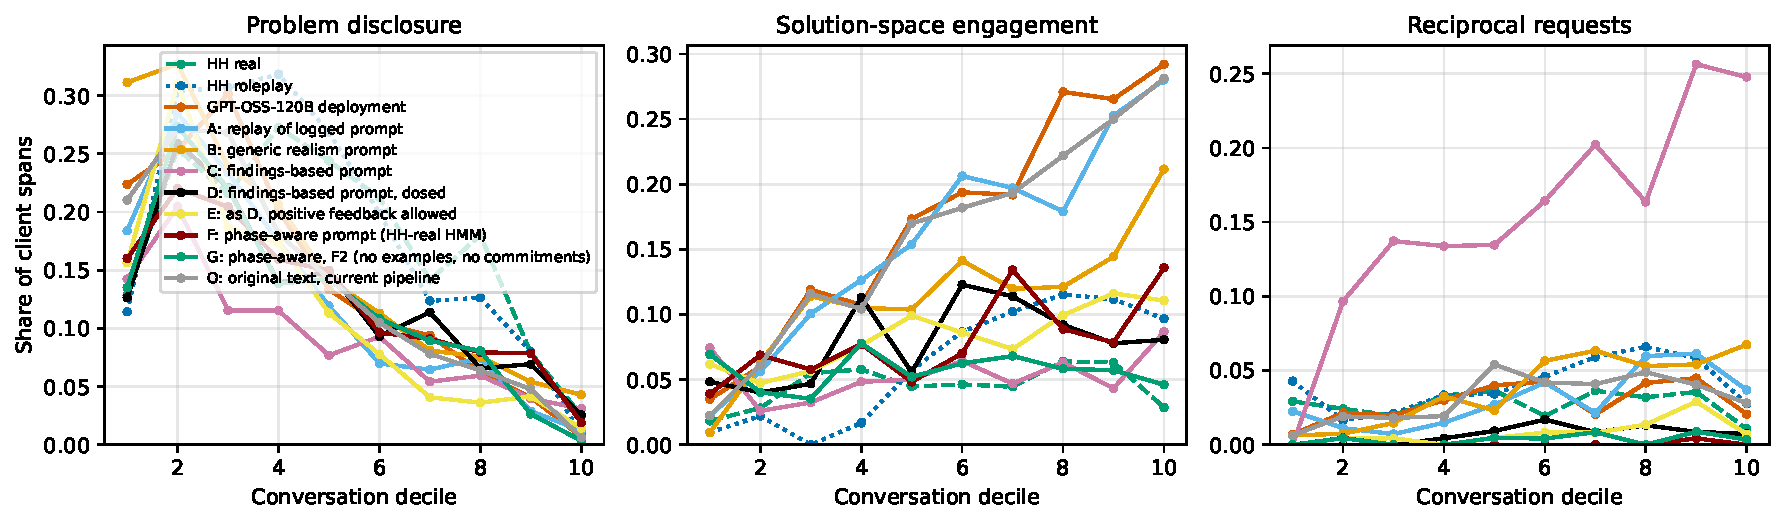
\includegraphics[width=0.98\linewidth]{results/figures/oncoco/prompt_replay_deciles.pdf}
\caption{Client-side decile profiles of the replay arms next to the human conditions: share of client spans on problem disclosure, solution-space engagement, and general requests per conversation decile.}
\label{Sfig:replay-deciles}
\end{figure}

\section{Human Validation on the Study Corpora}
\label{Ssec:validation}
This section reports the expert validation of the OnCoCo classifier referenced in Sections~4.2, 5.5.2, and~7 of the main paper.

\textbf{Setup.} Both human corpora carry expert annotation under the OnCoCo scheme, produced by two different annotation teams: 4{,}354 units in 64 HH roleplay conversations and 3{,}591 chat units in 54 HH real conversations, the latter exported from MAXQDA and reconstructed from the source documents paragraph by paragraph. The experts segment by function and the pipeline by sentence, and the two cuts rarely coincide (boundary F1 0.13 on HH roleplay). We therefore re-classified the experts' own units with the pipeline's role prefix, so that the comparison holds the segmentation fixed and only the labels differ. No simulated-client conversation has expert annotation.

\textbf{Agreement.} Table~\ref{Stab:human-validation} gives unit-level agreement per corpus and role. Both corpora lie far below the in-domain figures of the OnCoCo test set (accuracy 0.79, model-to-human $\kappa$=0.88) and below the human intercoder agreement of the scheme ($\kappa$=0.84). HH real is the harder corpus throughout, with $\kappa$=0.34 against 0.45, and on its client side the classifier does not beat the majority baseline, because \emph{Problem statement} makes up 39\% of the units there and is recalled at 0.22. At the level of the scheme's pillars both corpora reach 0.81 to 0.82, so the broad field of action is recognized and the fine category is not. The classifier is too generous rather than blind: on the counselor side it uses 50 categories where the annotators use 33 to 35, and every category the annotators never use is by construction an error. The single largest confusion is \emph{Problem statement} against \emph{Problem definition}, 197 units in both directions in HH real and 90 in HH roleplay, with \emph{Own emotional expression} as the third member of the same family, and merging only these three labels raises the client-side $\kappa$ from 0.48 to 0.55 on HH roleplay and from 0.33 to 0.45 on HH real. A tolerant reading that merges neighbouring categories (backchannel against residual, consent against positive feedback, reflection types, question types, and the problem family) raises $\kappa$ to 0.62 on HH roleplay and 0.54 on HH real. That is the most generous figure obtainable, not the strictest, and every analysis that reports single categories is bound by the strict one.

\textbf{Signature categories.} Table~\ref{Stab:human-validation-categories} gives precision, recall, and F1 for the categories that carry the signatures of Section~5.2 in the main paper, next to the shares the experts and the classifier assign. \emph{Consent}, \emph{General request}, and \emph{Rejection} are the best-identified categories in both corpora. The largest error is the under-detection of \emph{Problem statement} in HH real (recall 0.22, expert share 0.202 against 0.068 for the classifier). Table~\ref{Stab:human-validation-buckets} pools the categories into the three client-side buckets of Section~5.2. Reciprocal requests are measured almost without loss (0.94 of the expert share in both corpora), solution-space engagement in the same direction with a rough match of the shares, and problem disclosure is over-reported by 15\% in HH roleplay and under-reported by 34\% in HH real. The units the classifier loses from the problem bucket do not move within the bucket but leave it, mostly to \emph{Consent}, the residual categories, and \emph{Own emotional expression}. Short units carry most of this loss (recall 0.09 at one to three words against 0.69 at 26 words and more), but length explains only a sixth of the gap between the corpora. The classifier is worse on real counseling in every length class.

\textbf{Distance compression.} With expert labels on both human corpora, the distance between them can be computed twice on identical units. Under expert labels the client-side JSD between HH roleplay and HH real is 0.359 [0.333, 0.402], under classifier labels 0.196 [0.182, 0.244], and the pipeline's own SaT spans give 0.233, so the unit is not the cause. A paired conversation-level bootstrap puts the compression at 0.163 [0.113, 0.197] on the client side and 0.140 [0.107, 0.160] over both roles. Within HH real, where one team and one codebook apply, the same comparison between the three regional services shows no compression (0.012 to 0.056, all intervals including zero). Two readings remain open: the classifier compresses exactly this contrast, or part of the expert distance is a codebook and team difference between the two annotation groups. We therefore read the result as a direction and not as a clean attenuation estimate. In either reading the classifier measures the distance between the two human conditions smaller than the experts do. Whether the same holds for the distance to simulated clients is the open question below.

\textbf{What the validation cannot settle.} The H--LLM term of $\Delta$ has no expert labels. If the classifier compresses the distance from real counseling to simulated clients by the same amount as the distance to human roleplay, $\Delta_{\mathrm{CL}}$ is unchanged. If it compresses it less, because simulated text is closer to the register of the training material, $\Delta_{\mathrm{CL}}$ shrinks. A stratified sample of about 400 expert-coded simulated-client units would close this gap.

\textbf{Repair attempts.} Three changes to how the classifier is fed do not repair the loss on HH real. Prefixing the preceding counselor turn collapses accuracy to 0.08, because 66\% of the predictions then come from the other role's inventory. Prefixing the client's own preceding unit raises problem recall from 0.47 to 0.53 but lowers accuracy from 0.36 to 0.26, because the model copies the previous label. Merging units of at most three words into the following unit moves the recall from 0.47 to 0.48 and the between-corpus contrast by 0.001. The bias is a property of the model, and a fix would need retraining with a context field.

\textbf{Inappropriate remark.} The category is a lexical artifact. Apology formulas (``tut mir leid''), prescriptive phrasing (``du musst''), absolute words (``niemand''), and generalizations trigger it at 6 to 10 times the base rate, and the four strongest triggers occur in none of the 49 units the experts themselves coded as inappropriate. The classifier marks assertive counselor speech, that is assessments, advice, and reassurance delivered in an informal register, as inappropriate, which is why the primary exclusion set of Section~\ref{Ssec:exclusions} removes the category.

\begin{table}[t]
\centering
\small
\begin{tabular}{lrrrrrrrrrr}
\hline
Condition and role & Units & Cat. & Words & Acc. & Base & $\kappa$ & Macro F1 & Wtd. F1 & Pillar & Group \\
\hline
HH roleplay -- all units & 4,354 & 61 & 10 & 0.461 & 0.089 & 0.445 \footnotesize[0.427, 0.464] & 0.344 & 0.464 & 0.817 & 0.621 \\
HH roleplay -- counselor & 2,467 & 33 & 11 & 0.418 & 0.158 & 0.388 \footnotesize[0.367, 0.411] & 0.319 & 0.429 & 0.778 & 0.565 \\
HH roleplay -- client & 1,887 & 28 & 9 & 0.517 & 0.151 & 0.481 \footnotesize[0.453, 0.509] & 0.381 & 0.516 & 0.869 & 0.694 \\
HH real -- all units & 3,591 & 59 & 10 & 0.360 & 0.202 & 0.339 \footnotesize[0.319, 0.358] & 0.304 & 0.371 & 0.813 & 0.623 \\
HH real -- counselor & 1,727 & 35 & 10 & 0.330 & 0.142 & 0.303 \footnotesize[0.277, 0.332] & 0.301 & 0.323 & 0.765 & 0.576 \\
HH real -- client & 1,864 & 24 & 9 & 0.387 & 0.389 & 0.332 \footnotesize[0.297, 0.370] & 0.313 & 0.419 & 0.857 & 0.666 \\
\hline
\end{tabular}
\caption{Agreement of the OnCoCo classifier with the expert annotation of the two human chat corpora. Both label sets sit on identical units: the classifier was re-run on the human segments, with the role prefix the pipeline uses, so only the labels differ and not the segmentation. \emph{Units} counts annotated segments, \emph{Cat.} the number of distinct OnCoCo categories the human annotators used in that block (the classifier can choose among 68, of which 66 have a counterpart in the German scheme), and \emph{Words} their median length in whitespace-separated tokens. \emph{Acc.} is unit-level agreement and \emph{Base} the share of the largest human category, the accuracy a constant prediction would reach. $\kappa$ is Cohen's kappa with a 95\% conversation-level bootstrap interval (2{,}000 draws). \emph{Macro F1} averages over the categories the humans used, so rare ones weigh as much as frequent ones, while \emph{Wtd. F1} weighs by support. \emph{Pillar} and \emph{Group} are accuracies after truncating both codes to their second and third field, that is to the broad field of action and to the function group within it.}
\label{Stab:human-validation}
\end{table}

\begin{table}[t]
\caption{Classifier against expert annotation for the categories that carry the signatures of Section~5.2 in the main paper, per human corpus. \emph{Exp.} and \emph{Model} are the shares of that role's units the experts and the classifier assign to the category, \emph{P}, \emph{R}, and \emph{F1} precision, recall, and F1 of the classifier against the experts. Client categories are shares of client units, counselor categories shares of counselor units. The counselor residual category does not exist in the German scheme of the HH roleplay annotation, so every unit the classifier places there is an error.}
\label{Stab:human-validation-categories}
\centering
\footnotesize
\setlength{\tabcolsep}{4pt}
\fitwidth{\begin{tabular}{lrrrrrrrrrr}
\toprule
& \multicolumn{5}{c}{HH roleplay} & \multicolumn{5}{c}{HH real} \\
\cmidrule(lr){2-6}\cmidrule(lr){7-11}
Category & Exp. & Model & P & R & F1 & Exp. & Model & P & R & F1 \\
\midrule
Problem statement & 0.051 & 0.046 & 0.53 & 0.49 & 0.51 & 0.202 & 0.068 & 0.64 & 0.22 & 0.32 \\
Problem definition & 0.031 & 0.047 & 0.26 & 0.41 & 0.32 & 0.010 & 0.072 & 0.00 & 0.03 & 0.01 \\
Consent & 0.065 & 0.081 & 0.71 & 0.88 & 0.78 & 0.038 & 0.063 & 0.58 & 0.96 & 0.72 \\
Rejection & 0.011 & 0.009 & 0.69 & 0.57 & 0.63 & 0.008 & 0.014 & 0.43 & 0.79 & 0.56 \\
General request & 0.029 & 0.028 & 0.78 & 0.73 & 0.76 & 0.022 & 0.021 & 0.75 & 0.71 & 0.73 \\
Other statements (client) & 0.002 & 0.018 & 0.08 & 0.75 & 0.14 & 0.009 & 0.037 & 0.18 & 0.74 & 0.29 \\
Other statements (counselor) & 0.000 & 0.052 & 0.00 & -- & 0.00 & 0.008 & 0.024 & 0.13 & 0.38 & 0.19 \\
Inappropriate remark (counselor) & 0.004 & 0.008 & 0.03 & 0.06 & 0.04 & 0.005 & 0.035 & 0.07 & 0.47 & 0.12 \\
\bottomrule
\end{tabular}
}
\end{table}

\begin{table}[t]
\caption{The three client-side signature buckets of Section~5.2 in the main paper under expert and classifier labels, on the experts' units. Shares are of client units with 95\% conversation-level bootstrap intervals, \emph{Ratio} is the classifier share over the expert share, and \emph{Recall} and \emph{Precision} are computed at bucket level, so a confusion inside the bucket does not count as an error.}
\label{Stab:human-validation-buckets}
\centering
\footnotesize
\setlength{\tabcolsep}{4pt}
\fitwidth{\begin{tabular}{llrrrrr}
\toprule
Bucket & Condition & Expert share [95\% CI] & Model share [95\% CI] & Ratio & Recall & Precision \\
\midrule
Problem disclosure & HH roleplay & 0.187 [0.170, 0.207] & 0.215 [0.195, 0.235] & 1.15 & 0.71 & 0.62 \\
Problem disclosure & HH real & 0.405 [0.366, 0.445] & 0.268 [0.233, 0.306] & 0.66 & 0.47 & 0.71 \\
Solution-space engagement & HH roleplay & 0.101 [0.085, 0.116] & 0.079 [0.066, 0.092] & 0.78 & 0.46 & 0.59 \\
Solution-space engagement & HH real & 0.062 [0.044, 0.085] & 0.069 [0.055, 0.083] & 1.11 & 0.33 & 0.30 \\
Reciprocal requests & HH roleplay & 0.068 [0.050, 0.087] & 0.064 [0.049, 0.079] & 0.94 & 0.73 & 0.78 \\
Reciprocal requests & HH real & 0.043 [0.028, 0.061] & 0.040 [0.027, 0.055] & 0.94 & 0.71 & 0.76 \\
\bottomrule
\end{tabular}
}
\end{table}

\section{Weighting and Persona-Matched Checks}
\label{Ssec:weighting}
Two further checks on the client-side proximity gap of Section~5.1 in the main paper (Table~\ref{Stab:weighting}). Pooled label proportions weight conversations by their length. Weighting every conversation equally instead, by averaging the per-conversation label distributions with explicit zeros for unused labels, moves $\Delta_{\mathrm{CL}}$ from 0.220 to 0.217. Restricting both roleplay conditions to the six personas that occur in HH roleplay and in H--LLM (40 and 220 conversations, persona identity as in Section~\ref{Sapp:personas}) moves it to 0.208, and equal weighting on the matched set gives 0.209. All intervals are conversation-level bootstraps with 5{,}000 resamples. Script: \texttt{analysis/semantic/oncoco/oncoco\_equal\_weight\_persona\_delta.py}.

\begin{table}[t]
\caption{Client-side proximity gap under equal conversation weighting and persona matching. JSD to HH real for H--LLM and HH roleplay, and their difference $\Delta_{\mathrm{CL}}$ with a 95\% conversation-level bootstrap interval. The first row reproduces the pooled result of the main paper.}
\label{Stab:weighting}
\centering
\footnotesize
\setlength{\tabcolsep}{4pt}
\fitwidth{\begin{tabular}{lrrrrrr}
\toprule
Variant & HH roleplay conv. & H--LLM conv. & JSD(real, H--LLM) & JSD(real, HH roleplay) & $\Delta_{\mathrm{CL}}$ [95\% CI] \\
\midrule
pooled spans (paper) & 68 & 414 & 0.453 & 0.233 & +0.220 [+0.178, +0.243] \\
equal-weighted conversations & 68 & 414 & 0.442 & 0.225 & +0.217 [+0.174, +0.239] \\
persona-matched, pooled spans & 40 & 220 & 0.458 & 0.251 & +0.208 [+0.160, +0.232] \\
persona-matched, equal-weighted & 40 & 220 & 0.450 & 0.241 & +0.209 [+0.159, +0.234] \\
\bottomrule
\end{tabular}
}
\end{table}

\section{Repeated Participation and Absolute Turn Positions}
\label{Ssec:participation}
This section checks two assumptions behind the intervals of Section~3.1 and the temporal signatures of Section~5.2 in the main paper.

\textbf{Repeated participation.} The 414 H--LLM conversations come from 281 students, identified by the platform's course-member account within each export. 202 students held one conversation, 39 two, 28 three, 10 four, and 2 five, and no student appears in more than one course or model. The main paper resamples conversations. Table~\ref{Stab:students} resamples students instead, so that all conversations of a student enter or leave a bootstrap sample together. HH real and HH roleplay are resampled by conversation in both columns, because the HH roleplays ran under a shared course account and repeated participation cannot be reconstructed there. Resampling students moves no interval bound by more than 0.004, and every per-model comparison of Figure~2 in the main paper keeps its reading. Script: \texttt{analysis/semantic/oncoco/oncoco\_student\_clustered\_bootstrap.py}.

\textbf{Absolute turn positions.} The deciles of Section~5.2 in the main paper place each client span relative to the client's own spans in that conversation. Real conversations are longer, with a median of 28 client turns against 18 in HH roleplay and 16 in H--LLM, so a decile covers more turns in HH real. Table~\ref{Stab:absolute-turns} therefore counts client turns in absolute terms, from the start and from the end of the conversation. A client turn is a maximal run of consecutive client messages, because the HH real export merges consecutive lines of one speaker while the other conditions keep them apart. Every signature holds. In the first three client turns, problem labels take 0.319 [0.302, 0.336] of H--LLM client spans against 0.122 [0.088, 0.158] in HH real and 0.173 [0.132, 0.216] in HH roleplay. In the last three client turns, solution-space labels take 0.368 [0.339, 0.396] against 0.029 [0.013, 0.046] and 0.094 [0.061, 0.132]. From the fourth client turn on, the H--LLM solution share is three to nine times the HH real share at the same turn, and it keeps rising in the 121 simulated conversations that run beyond 20 client turns. The H--LLM \emph{Rejection} share stays at or below 0.012 in every bin. Intervals are conversation-level bootstraps. Script: \texttt{analysis/semantic/oncoco/oncoco\_absolute\_turn\_profile.py}.

\begin{table}[t]
\caption{Conversation-resampled and student-resampled 95\% intervals for the proximity gaps and the per-model distances to HH real. Students are the platform's course-member accounts within each export. HH real and HH roleplay are resampled by conversation in both columns.}
\label{Stab:students}
\centering
\footnotesize
\setlength{\tabcolsep}{4pt}
\fitwidth{\begin{tabular}{lrrrcc}
\toprule
Quantity & Conv. & Students & Estimate & 95\% CI, conversations & 95\% CI, students \\
\midrule
$\Delta_{\mathrm{CL}}$ & 414 & 281 & +0.220 & [+0.178, +0.243] & [+0.177, +0.245] \\
JSD to HH real, GPT-OSS-120B, Client & 90 & 64 & 0.361 & [0.337, 0.402] & [0.338, 0.401] \\
JSD to HH real, Llama 3.3 70B, Client & 238 & 160 & 0.524 & [0.502, 0.553] & [0.500, 0.553] \\
JSD to HH real, Mixtral 8x7B, Client & 86 & 57 & 0.495 & [0.470, 0.529] & [0.468, 0.533] \\
$\Delta_{\mathrm{CO}}$ & 414 & 281 & +0.033 & [+0.000, +0.049] & [+0.000, +0.050] \\
JSD to HH real, GPT-OSS-120B, Counselor & 90 & 64 & 0.293 & [0.274, 0.338] & [0.273, 0.339] \\
JSD to HH real, Llama 3.3 70B, Counselor & 238 & 160 & 0.298 & [0.285, 0.330] & [0.285, 0.331] \\
JSD to HH real, Mixtral 8x7B, Counselor & 86 & 57 & 0.292 & [0.275, 0.337] & [0.275, 0.340] \\
\bottomrule
\end{tabular}
}
\end{table}

\begin{table}[t]
\caption{Client-side signature shares by absolute client turn, aligned at the start and at the end of the conversation. A client turn is a maximal run of consecutive client messages. Shares are of all client spans in the bin, pooled over conversations. Problem disclosure is \emph{Problem statement} and \emph{Problem definition}. Solution space is the feedback on recommendations, the report on their implementation, and the two resource-activation labels, as in Section~5.2 of the main paper.}
\label{Stab:absolute-turns}
\centering
\footnotesize
\setlength{\tabcolsep}{4pt}
\fitwidth{\begin{tabular}{llrrrrrrrrr}
\toprule
 & & \multicolumn{3}{c}{Problem disclosure} & \multicolumn{3}{c}{Solution space} & \multicolumn{3}{c}{Rejection} \\
\cmidrule(lr){3-5}\cmidrule(lr){6-8}\cmidrule(lr){9-11}
Aligned at & Client turn & HH real & HH roleplay & H--LLM & HH real & HH roleplay & H--LLM & HH real & HH roleplay & H--LLM \\
\midrule
Start & 1 & 0.020 & 0.116 & 0.226 & 0.000 & 0.007 & 0.012 & 0.000 & 0.007 & 0.002 \\
 & 2 & 0.163 & 0.222 & 0.357 & 0.022 & 0.009 & 0.033 & 0.000 & 0.009 & 0.000 \\
 & 3 & 0.195 & 0.200 & 0.445 & 0.034 & 0.011 & 0.028 & 0.011 & 0.032 & 0.006 \\
 & 4--6 & 0.335 & 0.347 & 0.333 & 0.033 & 0.030 & 0.096 & 0.033 & 0.023 & 0.007 \\
 & 7--10 & 0.246 & 0.257 & 0.199 & 0.058 & 0.051 & 0.204 & 0.023 & 0.033 & 0.005 \\
 & 11--15 & 0.203 & 0.153 & 0.107 & 0.050 & 0.098 & 0.310 & 0.040 & 0.022 & 0.007 \\
 & 16--20 & 0.208 & 0.090 & 0.106 & 0.056 & 0.064 & 0.358 & 0.023 & 0.021 & 0.007 \\
 & 21+ & 0.091 & 0.080 & 0.077 & 0.044 & 0.108 & 0.404 & 0.036 & 0.019 & 0.005 \\
\midrule
End & last & 0.039 & 0.000 & 0.014 & 0.000 & 0.021 & 0.345 & 0.008 & 0.000 & 0.002 \\
 & 2--3 from end & 0.027 & 0.044 & 0.032 & 0.048 & 0.133 & 0.380 & 0.016 & 0.006 & 0.012 \\
 & 4--6 from end & 0.134 & 0.098 & 0.102 & 0.086 & 0.109 & 0.313 & 0.034 & 0.025 & 0.005 \\
 & 7--10 from end & 0.190 & 0.198 & 0.221 & 0.051 & 0.096 & 0.207 & 0.045 & 0.029 & 0.008 \\
\bottomrule
\end{tabular}
}
\end{table}

\section{Held-out Replay}
\label{Ssec:heldout}
This section tests whether the dosed prompts of Section~5.7 in the main paper transfer to conversations they were not written for. Arms D and G were written and dosed on the 90 GPT-OSS-120B conversations. We applied both unchanged to the 117 Llama 3.3 70B conversations that ran under the same plain-text template family and passed the quality filter. 114 of them use personas that never occur in the GPT-OSS deployment. GPT-OSS-120B generates every arm with the settings of Section~\ref{Ssec:replay}, so arm A, the logged Llama prompt replayed by GPT-OSS-120B, is the baseline that isolates the prompt. Arm O passes the original Llama client text through the current pipeline. The arms were classified on a GPU node with the package versions of Table~\ref{Stab:parameters}, and that setup reproduces the local classification of arm O exactly (3{,}561 of 3{,}561 messages with identical spans and 5{,}417 of 5{,}417 identical span labels). Scripts: \texttt{analysis/prompt\_replay/} and \texttt{analysis/semantic/oncoco/oncoco\_prompt\_replay\_heldout.py}.

Both prompts transfer (Table~\ref{Stab:heldout}). The dosed rules lower the distance to HH real from 0.421 under the logged prompt to 0.287, and the phase-dependent rules to 0.253. Their proximity gaps are 0.054 [0.010, 0.089] and 0.020 [$-$0.024, 0.056], so the phase-dependent arm reaches the role-play level and the dosed arm stays slightly above it. The reduction against the logged prompt is larger than on the development conversations (0.134 and 0.169 against 0.093 and 0.112), where the logged prompt started closer to real counseling (0.326 against 0.421). The residual departures of the development set return. Positive feedback stays too rare (negative-to-positive ratios 7.32 and 2.15 against 0.78), early disclosure falls below the real level (0.074 and 0.095 against 0.128), and client-led entry into the help phase stays below the real-client rate (1.6\% and 0.7\% against 2.0\%). Both arms again lie farther from HH roleplay (0.327 and 0.309) than from HH real, so they reach the distance of a role-play partner by a different route, as on the development conversations.

\begin{table}[t]
\caption{Held-out prompt replay on the 117 Llama 3.3 70B conversations of the plain-text template family, client side. Arms A, D, and G are generated by GPT-OSS-120B on the original histories, and arm O is the original Llama text through the current pipeline. Columns as in Table~4 of the main paper, plus the JSD to HH roleplay. Intervals are conversation-level bootstraps with 20{,}000 resamples.}
\label{Stab:heldout}
\centering
\footnotesize
\setlength{\tabcolsep}{4pt}
\fitwidth{\begin{tabular}{lrrrrrrrrr}
\toprule
Group & JSD to HH real [95\% CI] & $\Delta$ [95\% CI] & JSD to roleplay & Problem d1 & Solution & Rej.\ conv. & Neg:Pos & Words & Entry \\
\midrule
HH real &  &  &  & 0.128 & 0.045 & 57\% & 0.78 & 10 & 2.0\% \\
HH roleplay & 0.233 [0.214, 0.278] & +0.000 [$-$0.035, +0.034] &  & 0.114 & 0.062 & 32\% & 0.43 & 12 & 4.0\% \\
\midrule
Llama 3.3 70B deployment (plain template) & 0.492 [0.471, 0.521] & +0.259 [+0.218, +0.283] & 0.398 & 0.163 & 0.149 & 8\% & 0.05 & 59 & 3.2\% \\
\midrule
O: original text, re-classified & 0.462 [0.441, 0.492] & +0.229 [+0.189, +0.254] & 0.369 & 0.193 & 0.142 & 8\% & 0.05 & 59 & 3.2\% \\
A: logged prompt, GPT-OSS & 0.421 [0.401, 0.452] & +0.188 [+0.146, +0.216] & 0.359 & 0.136 & 0.062 & 14\% & 0.18 & 26 & 5.0\% \\
D: dosed rules, unchanged & 0.287 [0.270, 0.321] & +0.054 [+0.010, +0.089] & 0.327 & 0.074 & 0.057 & 51\% & 7.32 & 8 & 1.6\% \\
G: phase-dependent rules, unchanged & 0.253 [0.236, 0.287] & +0.020 [$-$0.024, +0.056] & 0.309 & 0.095 & 0.047 & 68\% & 2.15 & 7 & 0.7\% \\
\bottomrule
\end{tabular}
}
\end{table}

\section{Pipeline and Generation Parameters}
\label{Ssec:parameters}
Table~\ref{Stab:parameters} lists the settings behind every number in the main paper. Code, prompts, and the adapter are in the companion repository.

\begin{table}[t]
\caption{Pipeline and generation parameters.}
\label{Stab:parameters}
\centering
\footnotesize
\setlength{\tabcolsep}{4pt}
\begin{tabular}{lp{0.72\linewidth}}
\toprule
Stage & Setting \\
\midrule
Segmentation & SaT-6l (\texttt{segment-any-text/sat-6l}) with a LoRA adapter (rank 128, alpha 256, dropout 0.1, attention query and value), boundary threshold 0.5, sliding windows of 512 tokens. wtpsplit 2.1.7, adapters 1.2.0. \\
Classification & XLM-RoBERTa-large fine-tuned on OnCoCo 1.0, the study checkpoint (68 output units, two of them counselor codes outside the 66-category scheme that are never predicted in the corpora), input prefixed with ``Counselor:'' or ``Client:'', no role masking of the output, batch size 16. transformers 4.51.3, torch 2.10.0. \\
Distance & Jensen--Shannon distance, square root of the base-2 divergence, over pooled span counts per condition and role. \\
Intervals & Percentile bootstrap over conversations, seed 42. 20{,}000 resamples for proximity gaps, per-model distances, student-clustered intervals, and replay arms on spans. 5{,}000 for replay arms on messages, weighting checks, and absolute turn positions. \\
Noise scale & Split-half band from 1{,}000 random halvings of HH real. Size-matched null from 1{,}000 draws with replacement at the compared sizes. \\
Transitions & 2{,}000 split-halves of HH real, two-sided empirical $p$ for off-diagonal cells with at least 10 transitions, Benjamini--Hochberg at $q=0.10$. \\
Phase model & Categorical HMM (hmmlearn 0.3.3), three states, 20 random initialisations with seeds 42 to 61, at most 500 EM iterations, tolerance $10^{-4}$, best log-likelihood kept. \\
Deployments & Logged sampling of the GPT-OSS-120B and Llama 3.3 70B deployments on a hosted inference service: temperature 1, at most 3{,}000 tokens, no frequency or presence penalty. The Mixtral 8x7B deployment logged neither prompts nor settings. \\
Replay & \texttt{openai/gpt-oss-120b} served with vLLM 0.28 on one A100 80\,GB, temperature 1, at most 3{,}000 tokens, no penalties, top-$p$ and reasoning effort at server defaults, no fixed seed, prompt sent as one user message, context length 16{,}384 tokens. \\
\bottomrule
\end{tabular}

\end{table}

\section{Client Sentiment Against Both Human Baselines}
\label{Ssec:sentiment}
This section reports the client sentiment behind the recommendation in Section~6 of the main paper. We scored every client message with the German sentiment model \texttt{oliverguhr/german-sentiment-bert}, the classifier that Tr\"ag et al. (2026) used for AI-guided debriefings. Table~\ref{Stab:sentiment} gives the shares per condition. Roleplay clients are about as positive as simulated clients. Both are more positive than real clients. We compared the positive share per conversation with two-sided Mann--Whitney tests. HH roleplay differs from HH real (Cliff's $\delta$=0.35, $p$=.001). H--LLM differs from HH real as well ($\delta$=0.29, $p<.001$). H--LLM and HH roleplay do not differ ($\delta$=0.05, $p$=.50).

\begin{table}[t]
\caption{Sentiment of client messages per condition. Shares of messages that \texttt{oliverguhr/german-sentiment-bert} classifies as negative, neutral, or positive.}
\label{Stab:sentiment}
\centering
\footnotesize
\begin{tabular}{lrrrr}
\toprule
Condition & Client messages & Negative & Neutral & Positive \\
\midrule
HH real & 1{,}632 & 0.586 & 0.170 & 0.244 \\
HH roleplay & 1{,}366 & 0.455 & 0.220 & 0.324 \\
H--LLM & 7{,}758 & 0.451 & 0.196 & 0.353 \\
\bottomrule
\end{tabular}
\end{table}

\end{document}
